%; whizzy chapter
% -initex iniptex -latex platex -format platex -bibtex jbibtex -fmt fmt
% 以上 whizzytex を使用する場合の設定。


%     Tokyo Debian Meeting resources
%     Copyright (C) 2010 Junichi Uekawa

%     This program is free software; you can redistribute it and/or modify
%     it under the terms of the GNU General Public License as published by
%     the Free Software Foundation; either version 2 of the License, or
%     (at your option) any later version.

%     This program is distributed in the hope that it will be useful,
%     but WITHOUT ANY WARRANTY; without even the implied warranty of
%     MERCHANTABILITY or FITNESS FOR A PARTICULAR PURPOSE.  See the
%     GNU General Public License for more details.

%     You should have received a copy of the GNU General Public License
%     along with this program; if not, write to the Free Software
%     Foundation, Inc., 51 Franklin St, Fifth Floor, Boston, MA  02110-1301 USA

%  preview (shell-command (concat "evince " (replace-regexp-in-string "tex$" "pdf"(buffer-file-name)) "&"))
% 画像ファイルを処理するためにはebbを利用してboundingboxを作成。
%(shell-command "cd image201002; ebb *.png")

%%ここからヘッダ開始。

\documentclass[mingoth,a4paper]{jsarticle}
\usepackage{monthlyreport}

% 日付を定義する、毎月変わります。
\newcommand{\debmtgyear}{2010}
\newcommand{\debmtgmonth}{2}
\newcommand{\debmtgdate}{20,21}
\newcommand{\debmtgnumber}{61}

\begin{document}
\begin{titlepage}
\thispagestyle{empty}

% タイトルページ:編集必要な部分は最初のマクロに飛ばすこと

\vspace*{-2cm}
第\debmtgnumber{}回 東京エリア Debian 勉強会資料

\hspace*{-2.4cm}
\includegraphics[width=210mm]{image200801/2008title.eps}\\
\hfill{}\debmtgyear{}年\debmtgmonth{}月\debmtgdate{}日

\end{titlepage}


\dancersection{Introduction}{上川 純一}

\begin{multicols}{2}
 
 
 今月のDebian勉強会へようこそ。これからDebianの世界にあしを踏み入れると
 いう方も、すでにどっぷりとつかっているという方も、月に一回Debianについ
 て語りませんか?

 Debian勉強会の目的は下記です。

 \begin{itemize}
 \item \underline{Debian Developer} (開発者)の育成。
 \item 日本語での「\underline{開発に関する情報}」を整理してまとめ、アップデートする。
 \item \underline{場}の提供。
 \begin{itemize}
  \item 普段ばらばらな場所にいる人々が face-to-face で出会える場を提供
	する。
  \item Debian のためになることを語る場を提供する。
  \item Debianについて語る場を提供する。
 \end{itemize}
 \end{itemize}		

 Debianの勉強会ということで究極的には参加者全員がDebian Packageをがりがり
 と作るスーパーハッカーになった姿を妄想しています。情報の共有・活用を通し
 て Debianの今後の能動的な展開への土台として、「場」としての空間を提供す
 るのが目的です。

\end{multicols}

\newpage

\begin{minipage}[b]{0.2\hsize}
 \definecolor{titleback}{gray}{0.9}
 \colorbox{titleback}{\rotatebox{90}{\fontsize{80}{80} {\gt デビアン勉強会} }}
\end{minipage}
\begin{minipage}[b]{0.8\hsize}
\hrule
\vspace{2mm}
\hrule
\tableofcontents
\vspace{2mm}
\hrule
\end{minipage}

\dancersection{事前課題}{上川 純一}

今回の事前課題は以下です:

\begin{enumerate}
 \item Debian について現在知っていることを教えてください。
 \item Debian について知りたいとおもっていることを教えてください。
 \item Debianを使う理由を挙げてください。
\end{enumerate}

この課題に対して提出いただいた内容は以下です。

\begin{prework}{ �����ϥ� }
\begin{enumerate}
\item �ϻϼԤ� Ian ����Ȥ��κ� Debra �����̾������̿̾���줿�� 
\item ���äѤ����ꤹ���ơ�������ˤ����ޤ�ʤ���
\item ���֤���ͳ�ϡ���ʬ�����ޤΤ��㤯�����餫�ʤ���
\end{enumerate}
\end{prework}
\begin{prework}{ emasaka }
\begin{enumerate}
\setcounter{enumi}{2}
\item �Ȥˤ�����������Υѥå��������鹽��������ǡ����뤤��ɬ�פ˱�����
      �ѥå��������ɲä��ơ��ʤ����Ĥ������ٰ¿����ơ����Ӥ˹�ä�������
      ����Ȥ������
\end{enumerate}
\end{prework}
\begin{prework}{ henrich }
\begin{enumerate}
\item dis���ʤ���⤬��Ф�򵤤ʥץ��������ȤǤ���
\item �ץ��������ȥ꡼�����γ�ư�����β����Ƥ�Ρ���
\item �ֱ郎���ä�����פǤ� :)
\end{enumerate}
\end{prework}
\begin{prework}{ mkouhei }
\begin{enumerate}
\setcounter{enumi}{2}
\item ʣ���Υ������ƥ�����Υޥ���򡢤��ΰ㤤�򵤤ˤ��������ѤǤ���ѥ�
      �����������ƥब���������뤿��Ǥ����Ȥ��Ϥ᤿���ä����Ǥ⤢��ޤ���
      �����ǻȤäƤ���Τ����Ǥ�5����Ǥ���
\end{enumerate}
\end{prework}
\begin{prework}{ ����(yy\_y\_ja\_jp) }
\begin{enumerate}
\setcounter{enumi}{2}
\item DFSG�����뤫�顥\&�ѥå������󥰥����ƥबͥ��Ƥ��뤫�顥�Ǥ��͡�
\end{enumerate}
\end{prework}
\begin{prework}{ ������ }
\begin{enumerate}
\setcounter{enumi}{2}
\item ������������ۤΥѥå��������������ƥ�˽в�ä��Ȼפäư��衢���äȻȤäƤޤ���
\end{enumerate}
\end{prework}


\dancersection{最近のDebian関連のミーティング報告}{上川純一}
\subsection{東京エリアDebian勉強会60回目報告}
% (query-replace-regexp "<.*?>" "")
% (query-replace-regexp "^[	 ]\+" "")

2010年の3月に次期安定版である コードネーム "squeeze" がリリースフリーズ
に入る予定です。 これに合わせて世界各地で Debian Bug Squashing Party が
行われます。 前回の 東京エリア Debian 勉強会は 勉強会をかねて、この Bug
 Squashing Party を東京大学先端科学技術研究センターに会場をお借りして実
施しました。

% =======================================================================
\dancersection{Debian の紹介}{やまねひでき}
\index{why debian}
% =======================================================================

\subsection{Debian とは何か}
「Debian とは一体何ですか? \footnote{\url{http://www.debian.org/intro/about}}」
には以下のように書かれています。

\begin{description}
\item \small Debian Project は、フリーなオペレーティングシステムを作成するために連携した
個人の集団です。 我々が作成したこのオペレーティングシステムは Debian GNU/Linux 
もしくはもっと短かく簡単に Debian と呼ばれています。
\end{description}

\subsection{Debian の特徴}
今だと Windows/MacOSX 以外の「いわゆるフリーなOS」はいくつかあります。
では、他の OS / ディストリビューションと Debian の違い、その特徴を語る
キーワードとは何でしょうか?私は「Universal OS」「フリー」「ボランティア」
の三つを挙げます。順を追って説明します。

\subsubsection{Universal OS}
これが Debian が目指すものです。その意味するところは
「あらゆるマシンで動くフリーなソフトウェアによる誰もが使えるOS」です。
単に PC で動くだけではなく、最近は廃れてきましたが UNIX ワークステーションや
汎用機、組み込み用機器、モバイル端末、ゲーム機…あらゆるマシンで動作すること
を目指しています。そのため多数の CPU アーキテクチャをサポートしているのが
特徴です。サポートする/した/しようとしているアーキテクチャは以下があります。

\begin{minipage}[t]{0.45\hsize}
\begin{itemize}
 \item i386	(通常の PC)
 \item amd64	(最近の 64bit CPU)
 \item ia64	(流行らない Intel の64bit CPU。Itanium など)
 \item mips/mipsel
 \item arm/armel(シャープの Netwalker やモバイル端末がこれ)
 \item alpha
\end{itemize}
\end{minipage}
\begin{minipage}[t]{0.45\hsize}
\begin{itemize}
 \item hppa	(HP のワークステーション)
 \item sparc	(Sun)
 \item powerpc
 \item m68k	(昔の Macintosh や Amiga など)
 \item s390 	(汎用機です)
 \item sh	(日立の)
 \item avr32
\end{itemize}
\end{minipage}

また、その動作の核となるカーネルも Linux だけではなく他のカーネルに取り替えても
動作することを目指しています。この移植版としては

\begin{itemize}
 \item Hurd	(永遠の開発版?)
 \item kfreeBSD (i386, amd64)\footnote{NetBSD, OpenBSD は途中で作業する人の気力が尽きているようです。}
\end{itemize}

があります。\footnote{残念ながら Plan9 はありませんが、その上で動くツール類は移植されています。}

単に動作する機器/カーネルが多いだけではなく、その上のユーザランドのソフトも豊富で、
パッケージ化されており導入が容易になっています。現在リリースされている Debian 5.0 
コードネーム「Lenny」ではその数は25,000パッケージを越え、その数はさらに増えつづけています。
Linux で使えるソフトウェアを探す場合、大抵は既に Debian のパッケージとして提供されているので
気軽に試すことができるでしょう。

それから Debian で利用可能な言語は多種に渡ります。それは自然言語(英語、日本語など)
でもあり、計算機言語という意味でもあります\footnote{計算機言語の話は後で別の方が
滔々としてくれるでしょう :-)}。巷ではマイナーと呼ばれるような言語であっても
「Universal OS」を目指す Debian は積極的に取り込んでいます。例えば、ブータン公用語
「ゾンカ語」をサポートする DzongkhaLinux は Debian をベースに開発され、その成果は 
Debian に取り込まれています\footnote{これは商用OSでは「採算にあわない」ので
サポートが遅れがちになる少数言語/民族にとっての希望の現れと言えるでしょう}。


\subsubsection{フリー}
Debian の考える「フリー」は単に無料に止まらず、Debian フリーソフトウェアガイドライン
 (DFSG) という形でまとまっており、これが元になって「オープンソース」が生まれました。
この点が担保される、この考えを皆が共有することでさらに豊かなソフトウェア/コンテンツ/社会が
生まれています。このフリーというのは考えてみると中々奥深いものがありますので、ぜひ DFSG 
には一度目を通した上で Debian の考えるフリーという意味について Debian Developer の方などと
話をしてみてください。

\subsubsection{ボランティア}
最後のキーワードです。Debian はその開発や財政基盤を会社や財団に持たない極めて稀有な
開発集団です。大抵の有名ディストリビューションが企業をバックに開発をしていたり財団を
持ってそのいたりする\footnote{Fedora ← Red Hat, openSUSE ← Novell, Ubuntu ← Canonical, 
OpenOffice.org ← Oracle (Sun), Firefox ← Mozilla Foundation/Corporation など}のですが、
Debian 自体は財団や企業を持ちません\footnote{寄付などのために Software Public Interest 
という別法人がいますが、これは Debian だけではなく PostreSQL なども支援しています}。
ボランティアが世界中でインターネットを介して開発するという状態が10年以上も続けられており、
その規模は1000人を優に越えています。

\subsection{誰が Debian を使っているの?}
では、実際に誰が Debian を使っているのでしょうか? 「仕事で使うなら Red Hat 
Enterprise Linux かそのクローンの CentOS が普通だよね〜」などと言い切っている人は
いませんか? 実は、世の中に Debian で実際のビジネスを回している企業は山のようにあります。
その中にはあなたが知っている企業もあるはずです。また、開発に愛用しているという方も
少なくありません。あなたが使っているソフト/サービスは実は Debian が動いている/ベースに
なっている…かも知れませんよ。

\subsection{最後に}
簡単ではありますが、Debian の紹介をさせて頂きました。
これも何かの縁だし Debian を使ってみてもいいかな、と多少でも思っていただければ幸いです。

\subsection{Debian フリーソフトウェアガイドライン}
Debian フリーソフトウェアガイドライン全文\footnote{\url{http://www.debian.org/social\_contract\#guidelines}}を掲載します。

\begin{figure}[h]
 {\small
\begin{enumerate}
 \item 「自由な再配布」…Debian システムを構成するソフトウェアのライセン
       スは、そのソフトウェアを、複数の異なる提供元から配布されているプ
       ログラムを集めたソフトウェア ディストリビューションの一部として、
       誰かが販売したり無料配布したりすることを 制限してはいけません。ま
       た、ライセンスはそのような販売に対して 使用料やその他の手数料を要
       求してはいけません。
 \item 「ソースコード」…プログラムにはソースコードが含まれていなければ
       ならず、 かつ実行形式での配布に加えてソースコードでの配布をも 許
       可していなければなりません。
 \item 「派生ソフトウェア」…ライセンスは、ソフトウェアの修正や派生ソフ
       トウェアの作成、並びにそれら をオリジナルソフトウェアのライセンス
       と同じ条件の下で配布することを認め ていなけばいけません。
 \item 「原作者によるソースコードの整合性維持」…ライセンスは、プログラ
       ムを構築時に変更する目的でパッチファイル をソースコードとともに配
       布することを容認している場合に限り、 ソースコードを修正済の形式で
       配布することを制限することができます。 この場合、そのライセンスは
       修正済のソースコードから構築されたソフトウェアの 配布を明示的に許
       可していなければなりません。 またライセンスは派生ソフトウェアにオ
       リジナルソフトウェアと異なる名前 を付けること、あるいは異なるバー
       ジョン番号を付けることを要求できます (これは妥協案です。Debian グ
       ループは全ての作者に、ファイル、 ソース、バイナリについての変更を
       制限しないよう奨めています)。
 \item 「すべての個人、団体の平等」…ライセンスは、すべての個人や団体を
       差別してはなりません。
 \item 「目標分野の平等」…ライセンスは、人々が特定の目標分野でプログラ
       ムを利用することを 制限してはいけません。たとえば、商用利用や、遺
       伝学の研究での プログラムの使用を制限していてはいけません。
 \item 「ライセンスの配布」…プログラムに付随する権利は、プログラムが再
       配布された すべての人々に対して、追加ライセンスの履行を必要とする
       ことなく、 適用されなければなりません。
 \item 「ライセンスは Debian に限定されない」…プログラムに付随する権利
       は、プログラムが Debian システムの 一部であるかどうかに左右されて
       はいけません。 プログラムが Debian から取り出され Debian とは別に
       使用 または配布されるとしても、その他の点でそのプログラムの ライ
       センス条項を満たしているならば、プログラムが再配布された すべての
       当事者は Debian システムにおいて付与されたのと 同じ権利を与えられ
       なければなりません。
 \item 「ライセンスは他のソフトウェアを侵害しない」…ライセンスは、その
       ソフトウェアとともに配布される他のソフトウェア に制約を加えてはな
       りません。たとえば、同じ媒体で配布される 他のソフトウェアがすべて
       フリーソフトウェアでなければならないと 要求してはいけません。
 \item 「フリーなライセンスの例」…GPL、BSD、および Artistic ライセンス
       は私たちがフリーと判断しているライセンスの例です。
\end{enumerate}
}
\caption{The Debian Free Software Guidelines (DFSG)}
\label{fig:dfsg}
\end{figure}

% =======================================================================
\dancersection{DebianのOCaml環境で開発する関数型言語インタプリタ}{日比野 啓}
\index{functional programming}
\index{OCaml}
\index{Haskell}
% =======================================================================

\subsection{OCamlはどんな言語}

静的型の型推論言語というのが今の私の認識です。
関数型言語らしい機能が注目されますが、それ以外のスタイルも良く利用されます。

ここではこの記事を読みすすめるにあたって必要そうなOCamlの機能について簡単に紹介します。

\subsubsection{値}

以下、対話環境の入出力を前提に話をすすめます。

ocaml-interpパッケージの /usr/bin/ocaml が対話環境のプログラムです。

\verb|# | は対話環境のプロンプトです。
ユーザーの入力の終わりを対話環境に認識してもらうために \verb|;;|を入力します。
なので対話環境の\verb|# |プロンプトの後ろから\verb|;;|までがユーザーの入力です。
\verb|- :|から始まる内容は対話環境の出力です。

\begin{commandline}
# 1;;
- : int = 1
# "abc";;
- : string = "abc"
# (1, "abc");;
- : int * string = (1, "abc")
# (1, ("abc", 2), 3);;
- : int * (string * int) * int = (1, ("abc", 2), 3)
# [ "a"; "b"; "c"];;
- : string list = ["a"; "b"; "c"]
# "a" :: "b" :: "c" :: [];;
- : string list = ["a"; "b"; "c"]
\end{commandline}

値を表す式を入力すると対話環境は型の名前と値を出力しています。
\verb|1|は\verb|int|型、\verb|"abc"|は\verb|string|型となっています。
対話環境に式を入力したので評価が行なわれ、その結果としての出力です。

\verb|(1, ("abc", 2), 3)|のようにコンマで区切って括弧でくくった値はタプルです。
値と値の組を表現できます。型の名前は \verb|*|で連ねます。任意の型の値を組にできる強力な機能です。

\verb|[ ]|でリストを表現することができます。また、\verb|::|はlispでいうところのconsです。
リストの要素は全て同じ型である必要があります。

\subsubsection{レコードとバリアント}

次は値を表現する前にあらかじめ型の定義が必要であるような値です。

\begin{commandline}
# type vec_2d = { x : int; y : int };;
type vec_2d = { x : int; y : int; }
# { x = 1; y = 2 };;
- : vec_2d = {x = 1; y = 2}
# type int_or_string_or_none = I of int | S of string | N;;
type int_or_string_or_none = I of int | S of string | N
# I 3;;
- : int_or_string_or_none = I 3
# S "hello";;
- : int_or_string_or_none = S "hello"
# N;;
- : int_or_string_or_none = N
\end{commandline}

一つ目の例はレコードです。Cの構造体のようなもので、フィールド名とフィールドの型を定義に記述します。
\verb|vec_2d|というレコードの型を定義して、\verb|{ x = 1; y = 2 }|という値を評価させました。

二つ目はバリアントあるいは代数データ型と呼ばれている種類の型です。
\verb|int_or_string_or_none|という型を定義していて、
その値は Iというタグの付いたint か Sというタグの付いたstring か N というタグ のどれかということです。
このタグのことを{\bf コンストラクタ}と呼びます。

バリアントは再帰的な定義も可能で、この機能で簡単に木構造を表現できます。

\begin{commandline}
# type str_tree = Leaf of string | Tree of (str_tree * str_tree);;
type str_tree = Leaf of string | Tree of (str_tree * str_tree)
# Leaf "abc";;
- : str_tree = Leaf "abc"
# Tree (Leaf "a", Tree (Leaf "b", Leaf "c"));;
- : str_tree = Tree (Leaf "a", Tree (Leaf "b", Leaf "c"))
\end{commandline}

\subsubsection{関数}

次は関数を表現する値です。

\begin{commandline}
# (fun x -> x + 1);;
- : int -> int = <fun>
# (fun x -> x);;
- : 'a -> 'a = <fun>
\end{commandline}

\verb|(fun x -> x + 1)|は関数です。
型が\verb|int -> int|と出力されていますが、
これはintを受けとってintを返す関数という意味です。
\verb|+|の引数はintとintなので結果として\verb|x|は\verb|int|、
\verb|fun x -> x + 1| は \verb|int -> int|というように型の推論が行なわれています。

二番目の\verb|(fun x -> x)|も関数です。
型が\verb|'a -> 'a|と出力されていますが、
これは何かある型の値を受けとって、同じ型の値を返す関数という意味です。
この \verb|'a -> 'a| の関数は任意の型に対して適用が可能なので、
全ての型についてこの関数が定義されている(\verb|int -> int| も \verb|string -> string| も ... etc)のと同様の効果があります。
このような型を多相型と呼びます。

\subsubsection{束縛}

\verb|let|を使って値を変数に束縛します。
以下は\verb|v|にたいして整数を\verb|f|に対して関数を束縛しています。

\begin{commandline}
# let v = 123;;
val v : int = 123
# v;;
- : int = 123
# let f x y = (x + y) * (x - y);;
val f : int -> int -> int = <fun>
# f 5 3;;
- : int = 16
\end{commandline}

\subsubsection{パターン照合}

OCamlは値の構造を分解しつつ変数を束縛することができます。
次の例ではタプルを分解して束縛を行なっています。

\begin{commandline}
# let (x, y) = (2, 3 + 4);;
val x : int = 2
val y : int = 7
# let (a, (b, c)) = (1, (2, 3));;
val a : int = 1
val b : int = 2
val c : int = 3
\end{commandline}

\verb|match ... with|を使用すると、構造分解を試みつつ条件分岐することができます。

関数\verb|len|はリストが空かどうかを判定しながら再帰しています。
束縛の定義時に自身の定義を使用するときには\verb|let|ではなく\verb|let rec|を使います。

関数\verb|what|は先程定義したバリアント\verb|int_or_string_or_none|の値の種類によって返す文字列を変えています。

関数\verb|get_int|は\verb|int_or_string_or_none|がintのときだけSome intを返し、そうでないときは None を返します。
'a option は組み込みの型で、ある型の値が有るかあるいは無いかを表現できるバリアントです。

\begin{commandline}
# let rec len ls = match ls with [] -> 0 | x :: rest -> 1 + len rest;;
val len : 'a list -> int = <fun>
# len [1; 2; 3];;
- : int = 3
# let what v = match v with I _ -> "int" | S _ -> "string" | N -> "none";;
val what : int_or_string_or_none -> string = <fun>
# what (S "abc");;
- : string = "string"
# what N;;
- : string = "none"
# let get_int v = match v with I i -> Some i | _ -> None ;;
val get_int : int_or_string_or_none -> int option = <fun>
# get_int N;;
- : int option = None
# get_int (I 10);;
- : int option = Some 10
\end{commandline}

\subsubsection{モジュール}

プログラムの規模がおおきくなってくると名前空間が重要になってきます。
OCamlにはmoduleの機能があり名前空間を分けることができます。
あるコンパイル単位がxyz.mlというファイル名だった場合、
その中の定義はXyzというmoduleの中に配置されます。
モジュール内にたとえばabcという名前があった場合、
公開されていれば他のコンパイル単位のファイルからも Xyz.abc という名前でアクセスすることができます。

\begin{commandline}
(* xyz.ml *)
let abc = "abc"
...


(* 他のファイル *)
... Xyz.abc ...
\end{commandline}

moduleの中にさらにmoduleを定義することもできます。
xyz.mlの中に作ったmodule SubXyzは、Xyz.SubXyzという名前のmoduleです。

定義済みのモジュールを使ってmoduleを定義することもできます。
組み込みのmoduleであるListを使って Xyz.L を定義しています。

\begin{commandline}
(* xyz.ml *)
module SubXyz =
  struct
  ...
  end

module L = List
\end{commandline}


\subsection{関数型言語のインタプリタの簡単な作りかた}

関数型言語とは何でしょうか。
ここでは関数を値としてあつかえる言語ということにして、
そのような言語のインタプリタを作る話をします。

\subsubsection{環境を渡すナイーブなインタプリタ実装}
\label{sec:envmach}

\paragraph{letの環境} \ 

例えば以下のようなプログラムを考えます。

\begin{commandline}
;; scheme function
(define (f)
  ;; env A
  (let ((x 1) (y 2) (z 3))
    ;; env B
    (let ((y 4))
      ;; env C
      (let ((z 5))
	;; env D
	(+ x y z)))))
\end{commandline}

\begin{commandline}
(* OCaml function *)
let f () =
  (* env A *)
  let (x, y, z) = (1, 2, 3) in
    (* env B *)
  let y = 4 in
    (* env C *)
  let z = 5 in
    (* env D *)
    x + y + z
\end{commandline}

変数の値の解決のためのテーブルを環境(environment)と呼ぶことにして、
次の図ような構造になっていると考えてみます。
変数の検索は上から下に行なわれるとすると、
それぞれのコメントの位置の環境は矢印の位置を参照していると考えてよいはずです。

 \includegraphics[height=0.3\hsize]{image201002/caml-env00.eps}\label{fig:env00}

\paragraph{関数呼び出しにおける環境} \ 

さらに以下のようなプログラムを考えます。

\begin{commandline}
(define (f x y)
  ;; env f
  (* x y 2))

;;env X

(let ((x 1) (y 2))
  (define (g)
    ;; env g
    (f 3 4))
  (g))

;;; may be another call of (f x y)
\end{commandline}

\begin{commandline}
let rec f x y =
  (* env f *)
  x * y * 2

(* env X *)

let (x, y) = (1, 2)
let rec g () =
  (* env g *)
  f 3 4

let v = g ()

(* may be another call of f x y *)
\end{commandline}

するとそれぞれのコメントの位置の環境は次の図のようになっているはずです。

 \includegraphics[height=0.25\hsize]{image201002/caml-env005.eps}

ここで環境Xは同じ環境なので、共有させることにすると次のような構造を考えることができます。
ここで注意する必要があるのは、環境fは関数fが呼び出される度に異なるということです。
fの定義位置である環境Xは共通ですが、環境fは関数fが呼び出される度に環境Xを指す環境を伸長する必要があります。

 \includegraphics[height=0.5\hsize]{image201002/caml-env01.eps}

\paragraph{クロージャの環境} \ 

以下のようなプログラムを考えます。

\begin{commandline}
(define h
  (let ((x 1) (y 2))
    ;; env c
    (let ((f (lambda (z)
               ;; env l
	       (+ x y z))))
      f)))

;; env X

(h 3)
;;; may be another call of (h x)
\end{commandline}

\begin{commandline}
let rec h =
  let (x, y) = (1, 2) in
  (* env c *)
  let f z =
    (* env l *)
    x + y + z
  in f

(* env X *)

let v = h 3
(* may be another call of h x *)
\end{commandline}

関数が変数hに束縛されています。
しかもhはx, yを束縛しているletの外側にあるにもかかわらず、
呼び出した際にはx, yの値を評価します。

このletのような機能をレキシカルスコープと呼び、
またこのような関数をレキシカルクロージャ(lexical closure)あるいは単にクロージャ(closure)と呼びます。

上の例での環境を考えてみると次のような構造になっているはずです。

 \includegraphics[height=0.5\hsize]{image201002/caml-env015.eps}

hに束縛されているclosureはあきらかに環境cを知っている必要があります。
なぜなら呼び出し時には環境cを指す環境を生成しなければならないからです。
したがってclosureは以下のような構造になっていると考えることができます。
envはclosureの定義位置の環境でargsは仮引数リストそしてbodyは関数本体の式です。

 \includegraphics[height=0.4\hsize]{image201002/caml-env02.eps}

式の評価に必要な環境を評価器内で渡しながら、
letや関数呼び出しの際には環境を伸長する方針を取ると、
比較的簡単にインタプリタを実装することができます。
また、環境を保持する構造を考えればclosureを実現することもできます。

 参考資料: \verb|http://www.sato.kuis.kyoto-u.ac.jp/~igarashi/class/isle4-05w/text/eopl003.html|

\subsection{OCamlでのlexingとparsing - ocamllexとocamlyacc}

\subsubsection{ocamllex}

ocamllexはOCamlに付属している字句解析関数生成器(lexer generator)で、
OCamlから呼び出せるlexerを生成してくれます。
以下のようにC言語でもおなじみの lex, flex と似たような使用感になっています。

\begin{commandline}

{
  (* header *)
  (* Lexingのルール部分で参照したい内容をOCamlで書く *)
}

(* 文字列パターンの定義 *)

(* 字句解析(lexing)のルール記述 *)

{
  (* trailer *)
  (* ルール部分で生成された関数を参照する内容をOCamlで書く *)
}

\end{commandline}

\subsubsection{ocamlyacc}

同様に、ocamlyaccはOCamlに付属している構文解析関数生成器(parser generator)で、
OCamlから呼び出せるparserを生成してくれます。
こちらもやはり、以下のように yacc, bison と似たような使用感になっています。

\begin{commandline}

%{
  (* header *)
  (* 構文木生成処理で参照したい内容をOCamlで書く *)
%}
  /* declarations */
  /* 終端記号の型や構文木のrootの宣言 */
%%
  /* rules */
  /* 文脈自由文法と構文木生成処理を記述 */
%%
  (* trailer *)
  (* 生成されたparserの関数を参照する内容をOCamlで書く *)

\end{commandline}

\subsubsection{ocamllexとocamlyaccの使用例}

ocamllexとocamlyaccを併用する場合には、
ocamlyaccで生成させたparserの終端記号の定義を
lexerから参照させるようにするのがもっとも単純な使い方です。

以下がS式parserを生成させる例です。
sParser.mlyをocamlyaccで処理するとsParser.mlが生成され、
sLexer.mllをocamllexで処理するとsLexer.mlが生成されます。

\par
\paragraph{sParser.mly}
型ごとに終端記号を\%tokenで宣言し、
\%startと\%typeで構文木のrootとその型を指定します。
rootの名前が構文解析関数の名前になります。

yaccと同じ要領で文脈自由文法を記述していきます。
exprは真偽値、数値、文字列であるか、
あるいは、exprドット対またはexprを並べたもの を括弧で括ったものという定義になっています。

\begin{commandline}

%{
  (* sParser.mly *)

  module C = SCons

%}

/* File sparser.mly */
%token LPAREN RPAREN DOT_SYMBOL EOL BOOL_TRUE BOOL_FALSE
%token <SCons.s_int> INT
%token <float> FLOAT
%token <string> SYMBOL
%token <string> STRING
%start expr
%type <SCons.s_expr> expr
%%

expr_list:
  { C.Null }
| expr DOT_SYMBOL expr { C.Cons($1, $3) }
| expr expr_list { C.Cons($1, $2) }

expr:
| BOOL_TRUE               { C.Bool(true) }
| BOOL_FALSE              { C.Bool(false) }
| INT                     { C.Int($1) }
| FLOAT                   { C.Float($1) }
| SYMBOL                  { C.Symbol($1) }
| STRING                  { C.String($1) }
| LPAREN expr_list RPAREN { $2 }

\end{commandline}

% $ dummy comment

\par
\paragraph{sLexer.mll}
文字列パターンの定義では、正規表現の要領で文字集合や繰り返しの表現を利用して
定義を作り、letで名前を付けていきます。文字を '' でくくる以外は正規表現と同様です。
定義した文字列パターンをさらに別の文字列パターンに再利用することができます。

ルール記述の部分では、tokenの文字列パターンとtoken生成式をlexの要領で記述していきます。
キーワードruleの後の文字列がlexerの関数名になります。なのでここではその関数の名前はtokenです。

字句解析(Lexing)の過程における入力ファイル内の位置は、
lexbufのlex\_start\_pに記号(token)の開始位置が、
lex\_curr\_pにtokenの終了の次の位置が保持されています。
ocamllexデフォルトの動作ではpos\_cnum フィールドが更新されるのみなので、
ファイル先頭からのバイト数しかわかりません。
陽に行数の認識やタブによるカラム数の補正を行なう場合には、
lex\_start\_pとtokenをもとにlex\_curr\_pを修正してやる必要があります。
\footnote{次のlex\_start\_pは現在のlex\_curr\_pから引き継がれるので、
lex\_curr\_pを修正すれば十分です。}



\begin{commandline}
{
  (* sLexer.mll*)

  module LX = Lexing
  module P = SParser
  ... (* 中略 *)
  let fix_position lexbuf =
    let newline pos = {
      pos with
	LX.pos_lnum = pos.LX.pos_lnum + 1;
	LX.pos_cnum = pos.LX.pos_cnum + 1;
	LX.pos_bol = pos.LX.pos_cnum + 1;
    } in

    let tab pos = {
      pos with
	LX.pos_cnum = pos.LX.pos_cnum + 8 - (pos.LX.pos_cnum - pos.LX.pos_bol) mod 8
    } in

    let other pos = {
      pos with
	LX.pos_cnum = pos.LX.pos_cnum + 1
    } in

    let rec fix_pos_rec pos str =
      let len = (String.length str) in
	match (if len > 0 then (Some (str.[0]), String.sub str 1 (len - 1))
	       else (None, "")) with
	    (None, _) -> pos
	  | (Some '\n', rest) -> fix_pos_rec (newline pos) rest
	  | (Some '\t', rest) -> fix_pos_rec (tab pos) rest
	  | (Some _, rest) -> fix_pos_rec (other pos) rest
    in
    let _ = lexbuf.LX.lex_curr_p <- fix_pos_rec (LX.lexeme_start_p lexbuf) (LX.lexeme lexbuf) in
      ()
}

/* 文字列パターンの定義 */
let str_esc = '\\'
let double_quote = '"'
let str_escaped_char = str_esc _
let str_char = [^ '\\' '"']
let str = double_quote (str_char | str_escaped_char)* double_quote

let left_paren = '('
let right_paren = ')'
let space = [' ' '\t' '\n' '\r']+
let dot_symbol = '.'
let bool_true  = '#' 't'
let bool_false = '#' 'f'

let int = '-'? ['0' - '9']+
let float = '-'? ['0' - '9']+ '.' ['0' - '9']* | '-'? ['0' - '9']* '.' ['0' - '9']+
let symbol = [^ '"' '(' ')' ' ' '\t' '\n' '\r']+

/* lexingのルール記述 */
rule token = parse
  | left_paren      { P.LPAREN }
  | right_paren     { P.RPAREN }
  | space      { fix_position lexbuf; token lexbuf }
  | dot_symbol      { P.DOT_SYMBOL }
  | bool_true       { P.BOOL_TRUE }
  | bool_false      { P.BOOL_FALSE }
  | int      { expr_integer (LX.lexeme lexbuf) }
  | float    { P.FLOAT(Pervasives.float_of_string(LX.lexeme lexbuf)) }
  | symbol   { P.SYMBOL(LX.lexeme lexbuf) }
  | str      { fix_position lexbuf; P.STRING(expr_string(LX.lexeme lexbuf)) }
  | eof      { raise Eof }

\end{commandline}

%\pagebreak

\subsection{HaskellのLexing}

Haskellには
ブロックの開始や終了のtokenや式の区切りのtokenを省略することができる
layout ruleという機能があります。
そのため省略されたtokenをlexingの過程で補ってやる必要があります。

まず、通常と同様にlexingを行なってtoken列を生成し、
そのtoken列に規則に従ってtokenを補うというように、2段階の工程を行ないます。

\subsubsection{layoutなしのLexing}

\paragraph{lexer0.mll header部分} \ 

まずは.mllのheader部分です。

後からlayout ruleにおいて必要となるカラム数を数えあげる処理ために位置情報の修正を行なう関数(fix\_position)を定義しています。
また、Haskellの文字および文字列リテラルはリテラル内のルールが複雑度の高い仕様なので、
別のlexer(後述)を呼び出しつつ実際の文字列表現を構成する関数(decode\_char, decode\_string)を準備しています。


\paragraph{fix\_position 位置情報の修正} \ 
\begin{commandline}
{
  (* lexer0.mll header部分 *)
  module LX = Lexing
  module P = Parser
  ... (* 中略 *)
  let fix_position lexbuf =
    let newline pos =
      { pos with
          LX.pos_lnum = pos.LX.pos_lnum + 1;
          LX.pos_cnum = pos.LX.pos_cnum + 1;
          LX.pos_bol = pos.LX.pos_cnum + 1;
      } in

    let tab pos =
      { pos with
          LX.pos_cnum = pos.LX.pos_cnum + 8 - (pos.LX.pos_cnum - pos.LX.pos_bol) mod 8
      } in

    let other pos =
      { pos with
          LX.pos_cnum = pos.LX.pos_cnum + 1
      } in

    let rec fix_pos_rec pos str =
      let len = (String.length str) in
        match (if len > 0 then (Some (str.[0]), String.sub str 1 (len - 1))
               else (None, "")) with
            (None, _) -> pos
          | (Some '\n', rest) -> fix_pos_rec (newline pos) rest
          | (Some '\t', rest) -> fix_pos_rec (tab pos) rest
          | (Some _, rest) -> fix_pos_rec (other pos) rest
    in
    let _ = lexbuf.LX.lex_curr_p <- fix_pos_rec (LX.lexeme_start_p lexbuf) (LX.lexeme lexbuf) in
      ()
  ... (* 中略 *)
\end{commandline}

\pagebreak

\paragraph{decode\_char, decode\_string 文字および文字列デコーダー} \
\begin{commandline}
  ... (* 中略 *)
  let decode_cexpr cexpr =
    let fchar = String.get cexpr 0 in
    let escexp = String.sub cexpr 1 ((String.length cexpr) - 1) in
    let fmatch exp str = Str.string_match (Str.regexp exp) str 0 in
      if fchar = '\\' then
        match escexp with
            "NUL"   -> Some '\x00'
          | "SOH" | "^A"   -> Some '\x01'
          | "STX" | "^B"   -> Some '\x02'
        ... (* 中略 *)
          | "RS"  | "^^"   -> Some '\x1e'
          | "US"  | "^_"   -> Some '\x1f'
          | "SP"           -> Some ' '

          | "\\"           -> Some '\\'
          | "\""           -> Some '"'
          | "'"            -> Some '\''

          | "DEL"          -> Some '\x7f'

          | _ when fmatch "^[0-9]+$" escexp
              -> Some (Char.chr (int_of_string escexp))
          | _ when fmatch "^[xX][0-9a-zA-Z]+$" escexp 
              -> Some (Char.chr (int_of_string ("0" ^ escexp)))
          | _ when fmatch "^[oO][0-7]+$" escexp
              -> Some (Char.chr (int_of_string ("0" ^ escexp)))

          | _ -> None

      else Some fchar

  let decode_char lexbuf =
    let cstr = LX.lexeme lexbuf in
    let len = String.length cstr in
      match decode_cexpr (String.sub cstr 1 (len - 2)) with
          Some c -> c
        | None   -> failwith (F.sprintf "Unkown char expression %s" cstr)

  let decode_string lexbuf =
    let sexpr = LX.lexeme lexbuf in
    let len = String.length sexpr in
    let strlbuf = Lexing.from_string (String.sub sexpr 1 (len - 2)) in
    let rec decode result =
      match HsStr.char strlbuf with
          HsStr.Eos -> result
        | HsStr.Char cstr ->
            if cstr = "\\&" then decode (result ^ "&")
            else decode (result ^ 
                           match (decode_cexpr cstr) with
                               None -> failwith (F.sprintf "Unkown char expression '%s' in literal string" cstr)
                             | Some c -> (String.make 1 c))
        | HsStr.Gap g -> decode result
    in decode ""
}
\end{commandline}

% $ dummy comment

\pagebreak

\paragraph{lexer0.mll 文字列パターン定義部分} \ 

次に文字列パターンの定義です。

行数はちょっと多いですが、特に難しいところはありません。
問題のリテラル文字列ですが、リテラル文字列部分の文字列パターン自体は問題なく表現できています。
しかし、リテラルで表現される文字列自体を復元するのが複雑なので前記および後述のような準備が必要になります。

\begin{commandline}
/* lexer0.mll 文字列パターン定義部分 */
let special = ['(' ')' ',' ';' '[' ']' '`' '{' '}']

let space = ' '
let newline = ("\r\n"|['\n' '\r'])
let tab = '\t'

let dashes = '-' '-' '-'*

let ascSmall = ['a'-'z']
let small = ascSmall | '_'
let ascLarge = ['A'-'Z']
let large = ascLarge

let plus = '+'
let minus = '-'
let exclamation = '!'
let ascSymbol_nbs = [ '!' '#' '$' '%' '&' '*' '+' '.' '/' '<' '=' '>' '?' '@' '^' '|' '-' '~' ]
let ascSymbol = ascSymbol_nbs | '\\'
let symbol = ascSymbol

let ascDigit = ['0'-'9']
let digit = ascDigit

let octit = ['0'-'7']
let hexit = ascDigit | ['a'-'z' 'A'-'Z']

let decimal = (digit)+
let octal = (octit)+
let hexadecimal = (hexit)+

let exponent = ['e' 'E'] ['+' '-']? decimal
let float = decimal '.' decimal exponent? | decimal exponent

let graphic = small | large | symbol | digit | special | [':' '"' '\'']
let any = graphic | space | tab

let comment = dashes ((space | tab | small | large | symbol | digit | special | [':' '"' '\'']) (any)*)? newline

let whitechar = newline | space | tab
let whitestuff = whitechar | comment 
let whitespace = (whitestuff)+

(*
let lwhitechar = space | tab
let lwhitestuff = lwhitechar | comment 
let lwhitespace = (lwhitestuff)+
*)

let char_gr = small | large | ascSymbol_nbs | digit | special | [':' '"']
let str_gr  = small | large | ascSymbol_nbs | digit | special | [':' '\'']

let charesc = ['a' 'b' 'f' 'n' 'r' 't' 'v' '\\' '"' '\'']
let str_charesc = charesc | '&'
let cntrl = ascLarge | ['@' '[' '\\' ']' '^' '_']
let gap = '\\' (whitechar)+ '\\'
(* let gap = '\\' (lwhitechar | newline)+ '\\' *)

let ascii = ('^' cntrl) | "NUL" | "SOH" | "STX" | "ETX" | "EOT" | "ENQ" | "ACK"
  | "BEL" | "BS" | "HT" | "LF" | "VT" | "FF" | "CR" | "SO" | "SI" | "DLE"
  | "DC1" | "DC2" | "DC3" | "DC4" | "NAK" | "SYN" | "ETB" | "CAN"
  | "EM" | "SUB" | "ESC" | "FS" | "GS" | "RS" | "US" | "SP" | "DEL"

let escape = '\\' ( charesc | ascii | decimal | 'o' octal | 'x' hexadecimal )
let str_escape = '\\' ( str_charesc | ascii | decimal | 'o' octal | 'x' hexadecimal )

let char = '\'' (char_gr | space | escape) '\''
let string = '"' (str_gr | space | str_escape | gap)* '"'

let varid = small (small | large | digit | '\'')*
let conid = large (small | large | digit | '\'')*

let varsym = symbol (symbol | ':')*
let consym = ':' (symbol | ':')*

let modid = conid
\end{commandline}

% $ dummy comment

\pagebreak

\paragraph{lexer0.mll ルール記述部分} \ 

最後にルール記述です。

スペース、タブ、改行などを含んでいるwhitespaceやstringのところで
fix\_positionを呼んで位置情報を補正しています。
またcharやstringのリテラルから文字や文字列を構成するために
decode\_char, decode\_string を呼び出しています。

\begin{commandline}
(* lexer0.mll ルール記述部分 *)
rule token = parse
  | '('  { P.SP_LEFT_PAREN(loc lexbuf) }
  | ')'  { P.SP_RIGHT_PAREN(loc lexbuf) }
  | ','  { P.SP_COMMA(loc lexbuf) }
  | ';'  { P.SP_SEMI(loc lexbuf) }
  | '['  { P.SP_LEFT_BRACKET(loc lexbuf) }
  | ']'  { P.SP_RIGHT_BRACKET(loc lexbuf) }
  | '`'  { P.SP_B_QUOTE(loc lexbuf) }
  | '{'  { P.SP_LEFT_BRACE(loc lexbuf) }
  | '}'  { P.SP_RIGHT_BRACE(loc lexbuf) }
      (** special tokens *)

  | "case"     { P.K_CASE(loc lexbuf) }
  | "class"    { P.K_CLASS(loc lexbuf) }
  | "data"     { P.K_DATA(loc lexbuf) }
  | "default"  { P.K_DEFAULT(loc lexbuf) }
  | "deriving" { P.K_DERIVING(loc lexbuf) }
  | "do"       { P.K_DO(loc lexbuf) }
  | "else"     { P.K_ELSE(loc lexbuf) }
  | "if"       { P.K_IF(loc lexbuf) }
  | "import"   { P.K_IMPORT(loc lexbuf) }
  | "in"       { P.K_IN(loc lexbuf) }
  | "infix"    { P.K_INFIX(loc lexbuf) }
  | "infixl"   { P.K_INFIXL(loc lexbuf) }
  | "infixr"   { P.K_INFIXR(loc lexbuf) }
  | "instance" { P.K_INSTANCE(loc lexbuf) }
  | "let"      { P.K_LET(loc lexbuf) }
  | "module"   { P.K_MODULE(loc lexbuf) }
  | "newtype"  { P.K_NEWTYPE(loc lexbuf) }
  | "of"       { P.K_OF(loc lexbuf) }
  | "then"     { P.K_THEN(loc lexbuf) }
  | "type"     { P.K_TYPE(loc lexbuf) }
  | "where"    { P.K_WHERE(loc lexbuf) }
  | "_"        { P.K_WILDCARD(loc lexbuf) }
      (** reservedid *)

  | ".."       { P.KS_DOTDOT(loc lexbuf) }
  | ":"        { P.KS_COLON(loc lexbuf) }
  | "::"       { P.KS_2_COLON(loc lexbuf) }
  | "="        { P.KS_EQ(loc lexbuf) }
  | "\\"       { P.KS_B_SLASH(loc lexbuf) }
  | "|"        { P.KS_BAR(loc lexbuf) }
  | "<-"       { P.KS_L_ARROW(loc lexbuf) }
  | "->"       { P.KS_R_ARROW(loc lexbuf) }
  | "@"        { P.KS_AT(loc lexbuf) }
  | "~"        { P.KS_TILDE(loc lexbuf) }
  | "=>"       { P.KS_R_W_ARROW(loc lexbuf) }
      (** reservedop *)

  | "as"              { P.K_AS(loc lexbuf) }  (** maybe varid *)
  | "qualified"       { P.K_QUALIFIED(loc lexbuf) }  (** maybe varid *)
  | "hiding"          { P.K_HIDING(loc lexbuf) }  (** maybe varid *)
  | varid      { P.T_VARID(LX.lexeme lexbuf, loc lexbuf) }
  | conid      { P.T_CONID(LX.lexeme lexbuf, loc lexbuf) }
      (** identifiers or may be qualified ones *)

  | whitespace  { fix_position lexbuf; P.WS_WHITE(loc lexbuf) }  (** comment begining with dashes is not varsym *)
      (** white spaces *)

  | plus       { P.KS_PLUS(loc lexbuf) }  (** maybe varsym *)
  | minus      { P.KS_MINUS(loc lexbuf) } (** maybe varsym *)
  | exclamation  { P.KS_EXCLAM(loc lexbuf) } (** maybe varsym *)
  | varsym     { P.T_VARSYM(LX.lexeme lexbuf, loc lexbuf) }
  | consym     { P.T_CONSYM(LX.lexeme lexbuf, loc lexbuf) }
      (** symbols or may be qualified ones *)

  | modid '.' varid   { P.T_MOD_VARID(decode_with_mod lexbuf, loc lexbuf) }
  | modid '.' conid   { P.T_MOD_CONID(decode_with_mod lexbuf, loc lexbuf) }
  | modid '.' varsym  { P.T_MOD_VARSYM(decode_with_mod lexbuf, loc lexbuf) }
  | modid '.' consym  { P.T_MOD_CONSYM(decode_with_mod lexbuf, loc lexbuf) }
      (** qualified xx *)

  | char      { P.L_CHAR(decode_char lexbuf, loc lexbuf) }
  | string    { fix_position lexbuf; P.L_STRING(decode_string lexbuf, loc lexbuf) }

  | decimal | ('0' ['o' 'O'] octal) | ('0' ['x' 'X'] hexadecimal)
        { P.L_INTEGER(Int64.of_string(LX.lexeme lexbuf), loc lexbuf) }

  | float      { P.L_FLOAT(float_of_string(LX.lexeme lexbuf), loc lexbuf) }

  | eof        { P.EOF(loc lexbuf) }
  ... /* 以下略 */
\end{commandline}


\paragraph{hsStr.mll} \ 

文字列のlexerです。

ここでのtokenは文字列リテラル内の1文字の表現あるいはギャップ(gap)です。
Haskellでは1つの文字列リテラルを中断して、
間に空白や改行やコメントを記述した後に、再開することができます。
この空白や改行やコメントの部分がgapです。

ここで定義されたchar関数を利用してdecode\_string関数は文字列を構成していくようになっています。

\begin{commandline}
{
  (* hsStr.mll *)
  module LX = Lexing

  type ct =
      Char of string
    | Gap of string
    | Eos
}

let special = ['(' ')' ',' ';' '[' ']' '`' '{' '}']

let space = ' '
let newline = ("\r\n"|['\n' '\r'])
let tab = '\t'

let ascSmall = ['a'-'z']
let small = ascSmall
let ascLarge = ['A'-'Z']
let large = ascLarge

let ascSymbol_nbs = [ '!' '#' '$' '%' '&' '*' '+' '.' '/' '<' '=' '>' '?' '@' '^' '|' '-' '~' ]

let ascDigit = ['0'-'9']
let digit = ascDigit

let octit = ['0'-'7']
let hexit = ascDigit | ['a'-'z' 'A'-'Z']

let decimal = (digit)+
let octal = (octit)+
let hexadecimal = (hexit)+

let lwhitechar = space | tab

let str_gr  = small | large | ascSymbol_nbs | digit | special | [':' '\'']

let charesc = ['a' 'b' 'f' 'n' 'r' 't' 'v' '\\' '"' '\'']
let str_charesc = charesc | '&'
let cntrl = ascLarge | ['@' '[' '\\' ']' '^' '_']
let gap = '\\' (lwhitechar | newline)+ '\\'

let ascii = ('^' cntrl) | "NUL" | "SOH" | "STX" | "ETX" | "EOT" | "ENQ" | "ACK"
  | "BEL" | "BS" | "HT" | "LF" | "VT" | "FF" | "CR" | "SO" | "SI" | "DLE"
  | "DC1" | "DC2" | "DC3" | "DC4" | "NAK" | "SYN" | "ETB" | "CAN"
  | "EM" | "SUB" | "ESC" | "FS" | "GS" | "RS" | "US" | "SP" | "DEL"

let str_escape = '\\' ( str_charesc | ascii | decimal | 'o' octal | 'x' hexadecimal )

rule char = parse
  | str_gr | space | str_escape  { Char(LX.lexeme lexbuf) }
  | gap                          { Gap(LX.lexeme lexbuf) }
  | eof                          { Eos }
\end{commandline}

% $ dummy comment

参考資料: \verb|http://www.sampou.org/haskell/report-revised-j/lexemes.html|

\subsubsection{Haskellのlayout rule}

この節の始めにも書いたようにlayout ruleは、
token列にさらにtokenを補ってやる処理です。
まずは補うルールを確認してみましょう。
以下に、Haskell 98 Language Reportの改訂版の和訳
\footnote{http://www.sampou.org/haskell/report-revised-j/syntax-iso.html\#layout}から引用してみます。

%%\paragraph{--- 引用ここから ---} \ 

\dotfill 引用ここから\dotfill

%% \par
%% \begin{tabular}{c|c|c}
%% \cline{1} & 引用ここから & \cline{3} \\
%% \end{tabular}

 レイアウトの影響は、この節では、レイアウトを用いているプログラムに、どのようにして、ブレースとセミコロンを追加するかを記述することによって指定する。この仕様は、変換を行う関数 L の形をとる。L  への入力は

\begin{itemize}

    \item この Haskell レポートの字句構文で指定されたような字句の並びで、以下のような追加トークンがついているもの。

    \begin{itemize}
          \item キーワード let、where、do あるいは of のあとに字句 \{ が続かない場合、トークン $\{n\}$ をキーワードの後に挿入する。ここで n は、もし次の字句があればそれのインデント、または、ファイルの終端に到達していれば 0 である。
          \item モジュールの最初の字句が \{ あるいは module では ないとき、その字句の前に $\{n\}$ を置く。ここで、n はその字句のインデントである。
          \item 同一行で、字句の開始の前には白空白しかないとき、この字句の前に $<n>$ を置く。ここで n はこの字句のインデントで、 前の二つの規則の結果、その前には $\{n\}$ が置かれていない。 (注意: 文字列リテラルは複数行にまたがることがある -- 2.6 節。したがって、
\begin{commandline}
              f = ("Hello \
                      \Bill", "Jake")
\end{commandline}
            では、\verb|\Bill| の前に $<n>$ は挿入されることはない。なぜなら、完全な字句の開始場所ではないからだ。また、, の前にも $<n>$ は置かれることはない。なぜなら、その前に 白空白以外のものがあるからだ。)
    \end{itemize}

    \item「レイアウト文脈」のスタックのそれぞれの要素は以下のどれかである。

    \begin{itemize}
          \item ゼロ、これは文脈を明示的に囲うこと(たとえばプログラマが開ブレース を用意した場合)を示す。もし最も内側の文脈が 0 なら、囲まれた文脈が 終了するか、新しい文脈がプッシュされるまで、レイアウトトークンは挿 入されない。
          \item 正の整数、これは囲まれたレイアウト文脈のインデントカラム数
    \end{itemize}

\end{itemize}

字句の「インデント」は字句の最初の文字のカラム数である。
ひとつの行のインデントとは最も左にある字句のインデントを表す。
このカラム数を決定するために以下のような規約をもつ固定幅のフォントを仮定する。

\begin{itemize}
    \item 改行、リターン、ラインフィードおよびフォームフィード文字はすべて新しい行を開始する
    \item 最初のコラムは 0 ではなく 1 である
    \item タブストップは8文字文ずつの位置にある
    \item タブ文字は現在位置から次のタブストップ位置までそろえるのに必要なだけの空白を挿入する。
\end{itemize}

レイアウトルールにあわせるために、ソースプログラム中の Unicode 文字は ASCII 文字と同じ幅の固定幅であると看倣す。しかしながら、見た目との混 乱を避けるためプログラマは暗黙のレイアウトの意味が非空白文字の幅に依 存するようなプログラムを書かないようにすべきである。

\paragraph{適用} \ 

L tokens [ ] は、tokens のレイアウトに関知しない変換をもたらす。
ここで、tokens はモジュールの字句解析および上述のようにカラム数表示子を追加した結果である。
L の定義は以下のとおり、ここでは 「:」をストリーム構築操作子として使い、「[ ]」は空のストリームである。

\begin{commandline}
L (<n>:ts) (m:ms)   = ; : (L ts (m:ms))  if m = n
                    = } : (L (<n>:ts) ms) if n < m
L (<n>:ts) ms       = L ts ms
L ({n}:ts) (m:ms)   = { : (L ts (n:m:ms)) if n > m   (Note 1)
L ({n}:ts) []       = { : (L ts [n]) if n > 0        (Note 1)
L ({n}:ts) ms       = { : } : (L (<n>:ts) ms)        (Note 2)
L (}:ts) (0:ms)     = } : (L ts ms)                  (Note 3)
L (}:ts) ms         = parse-error                    (Note 3)
L ({:ts) ms         = { : (L ts (0:ms))              (Note 4)
L (t:ts) (m:ms)     = } : (L (t:ts) ms) if m /= 0 and parse-error(t)  (Note 5)
L (t:ts) ms         = t : (L ts ms)
L [] []             = []
L [] (m:ms)         = } : L [] ms if m /=0           (Note 6)
\end{commandline}


%% \paragraph{Note 1.}

%% 入れ子になった文脈は、囲まれた文脈 ($n>m$) よりも深くインデ ントされていなければならない。
%% さもなければ、L は失敗し、また、コンパイラはレイアウトエラーを表示しなければならない。たとえば、

%% \begin{commandline}
%%   f x = let
%%            h y = let
%%     p z = z
%%                  in p
%%         in h
%% \end{commandline}

%% ここで、p の定義は囲まれた文脈のインデントよりも浅いインデントである。
%% この場合、h の定義によって設定される。

%% \paragraph{Note 2.}

%% where の後の最初のトークンが、たとえば、囲まれた文脈よりもインデントされているのでなければ、
%% そのブロックは空でなければならない。 
%% だから、空のブレースが挿入される。
%% トークン $\{n\}$ は $<n>$ に置き換 えられ、空のブレースが明示的になっていた場合の状況を模倣する。

%% \paragraph{Note 3.}

%% 現在のレイアウト文脈について 0 に対して照合することで、
%% 明示的な閉ブレースが明示的な開ブレースにのみ対応することを確かめる。
%% もし、明示的 な閉ブレースが暗黙の開ブレースに対応している場合には構文解析エラーとなる。

%% \paragraph{Note 4.}

%% これは、すべてのブレースの対は明示的なレイアウト文脈として扱われることを意味し、
%% ラベル付のデータ構築および更新 (3.15 節)を含む。ここにこの形式化と Haskell 1.4 での違いがある。

%% \paragraph{Note 5.}

%% 副次的な条件 parse-error(t) は次のように解釈される。
%% もし、次の トークンが t であるような L によって生成されたトークンが Haskell の文法の不正な接頭辞を表わしている場合、
%% および、 「\}」トークンが続く L によって生成さたトークンの Haskell 文法の正しい接頭辞である場合、parse-error(t) は真とな る。

%% $m /= 0$ のチェックは、暗黙に追加された閉ブレースが、暗黙の開ブレースに 対応することをたしかめる。

%% \paragraph{Note 6.}

%% 入力の終端において、保留された閉ブレースがすべて挿入される。
%% この時点 でレイアウト文脈のなかにある(すなわち、$m = 0$ である)とエラーとなる。


\dotfill 引用ここまで 以下略 \dotfill

だいぶ長くなってしまったので Note は省略です。

わかりにくいですが、ここでも内部的には2段階になっています。

まず元のtoken列に一つ目の操作を適用します。以下のような規則だと考えるとわかりやすいかもしれません。

\begin{itemize}
 \item let, where, do, of の後に \{ が無い場合には代わりにブロックの開始をあらわす token $\{n\}$ を挿入。
 \item ファイルの先頭もモジュール宣言が省略されていて \{ が無い場合には token $\{n\}$ でブロック開始。
 \item インデントのレベルで後からブロックを認識するために token $<n>$ を挿入しておく。
\end{itemize}

つぎに二つ目の操作である関数 L を適用します。

L はもとのtoken列とインデントレベルのスタックを引数にとり、
もとのtoken列にtokenを挿入したものを返す関数です。
やはり以下のような規則だと考えるとわかりやすいかもしれません。

\begin{itemize}
 \item インデントレベル$<n>$ が同じレベルのブロック内であれば(スタック参照) ; を挿入して式を終了、ブロックを継続
 \item インデントレベル$<n>$の方が浅ければ \} を挿入してブロックを終了
 \item インデントレベル$<n>$があって上のどちらでもなければ式を継続

 \item あるブロック内で(スタック参照)よりインデントレベルの深いブロック開始$\{n\}$があったら \{ を挿入しブロックを開始。
ブロック開始をあらわすインデントレベルnをスタックに積む
 \item ブロック開始 $\{n\}$ が最も外側でも同様にブロック開始。 \{ を挿入し、nをスタックに積む
 \item ブロック開始 $\{n\}$ があって上のどちらでもなければ \{ および \} を挿入し空のブロックを作る。
実はブロック開始ではなかったということがここでわかるので代わりに $<n>$ を挿入する。

 \item \} があったらスタックから 0 を取り出す
 \item \} があって 0 を降ろせなかったら parse error

 \item \{ があったらスタックに 0 を積む

 \item 上のどれでもなく、またブロック内であり、ブロックを継続すると parse error になるときは \} を挿入してブロックを閉じる。
 \item 上のどれでもなく、またブロック内であるときは parse error にならない限りブロックを継続。
 \item トークンもスタックも空ならおわり
 \item トークンが空でスタックに 0 でない値が残っているなら \} を挿入してスタックから取り出す。( 0があったらエラー )
\end{itemize}

参考資料: \verb|http://www.sampou.org/haskell/report-revised-j/syntax-iso.html#layout|


\paragraph{OCamlでの実装} \ 

「parse error にならない限りブロックを継続」のルールはかなり実装がやっかいでした。%%これはparserのところで後述します。
今回利用したocamlyaccはyaccやbisonと同じようにLALR(1)のparser generatorとなっており、
基本的にはtoken列を途中まで読み込んだ位置とそのtokenおよび一つ先のtokenによって構文解析中の次の動作を決定しています。
ここで出てきたような parse error になるまでブロックが閉じるかわからないような仕様とはあまり相性が良くありません。
backtrackを行なえるようなparserならこのような仕様に対してもより簡単に対応できると考えられます。
今回はtoken列のtokenごとにparse errorのフラグを付加してやりなおしを行なうことで対応しました。
実行効率はよくありませんが問題になるほどtoken数が多くならなければ大丈夫そうです。
将来的にはPackrat parsingのような方法でparserを書き直してみたいところです。

OCamlで上layout ruleを実装した関数が次のような感じです。
token列への一つ目の操作と二つ目の操作を順番に載せています。
P.BLK\_OPEN が $\{n\}$ で P.BLK\_LEVEL が $<n>$ にあたるものです。
もとの定義と似たよう記述で表現できているのがわかるでしょうか。

%%\paragraph{token列への操作 1つ目} \ 
\begin{commandline}
let all_token_rev_list lexbuf =
  let unget_s = S.create () in
  let get_token () = L0.token lexbuf in
  let blk_level_pair tk =
    let loc = L0.get_location tk in (loc.T.start_p.T.col + 1, loc) in
  let eof_token_p = (function P.EOF(_) -> true | _ -> false) in

  let rec scan_start () =
    match get_token () with
        (P.SP_LEFT_BRACE _ | P.K_MODULE _) as start -> start
      | P.WS_WHITE _ -> scan_start ()
      | other ->
          let _ = S.push other unget_s in
            P.BLK_OPEN (blk_level_pair other)
  in

  let scan_next prev = 
    let rec scan_next_rec () =
      let cur =
        if (S.is_empty unget_s) then (get_token ())
        else (S.pop unget_s) in

        match (prev, cur) with
            (_, (P.EOF(_) as eoft)) -> eoft
          | (_, P.WS_WHITE(_)) -> (scan_next_rec ())
          | ((P.K_LET(_) | P.K_WHERE(_) | P.K_DO(_) | P.K_OF(_)), (P.SP_LEFT_BRACE(_) as lbr)) -> lbr
          | ((P.K_LET(_) | P.K_WHERE(_) | P.K_DO(_) | P.K_OF(_)), tk) ->
              let (_, (level, loc)) = (S.push tk unget_s, blk_level_pair tk) in
                P.BLK_OPEN((if (eof_token_p tk) then 0 else level), loc)
          | (_, tk) ->
              let (_, loc) as p = blk_level_pair tk in
                if (loc.T.start_p.T.line
                    - (L0.get_location prev).T.end_p.T.line) > 0 then
                  let _ = S.push tk unget_s in P.BLK_LEVEL p
                else tk
    in (scan_next_rec ())
  in
    (LST.fold_left
       (fun r a -> ((a, new_err_flag ()) :: r))
       []
       (LST.create_stream (scan_start ()) scan_next eof_token_p))
\end{commandline}

%%\paragraph{token列への操作 2つ目} \ 
\begin{commandline}
let rec layout istream levels =
  let push_new_token tok lform =
    LST.Cons ((tok, new_err_flag ()), lform)
  in

  let (tok, err) =
    match LST.peek istream with
        None -> raise Parsing.Parse_error
      | Some x -> x
  in
    match (tok, levels) with
        ((P.BLK_LEVEL (n, loc)), (m :: mstl as ms)) when m = n ->
          let addtk = P.SP_SEMI(loc) in
            push_new_token addtk (lazy (layout (LST.tl istream) ms))
      | ((P.BLK_LEVEL (n, loc)), m :: ms) when n < m  ->
          push_new_token (P.SP_RIGHT_BRACE(loc)) (lazy (layout istream ms))
      | ((P.BLK_LEVEL (n, _)), ms)                         -> layout (LST.tl istream) ms
      | ((P.BLK_OPEN (n, loc)), (m :: ms as levels)) when n > m  ->
          push_new_token (P.SP_LEFT_BRACE(loc)) (lazy (layout (LST.tl istream) (n :: levels))) (* Note 1 *)
      | ((P.BLK_OPEN (n, loc)), []) when n > 0             ->
          push_new_token (P.SP_LEFT_BRACE(loc)) (lazy (layout (LST.tl istream) [n])) (* Note 1 *)
      | ((P.BLK_OPEN (n, loc)), ms)                        ->
          push_new_token
            (P.SP_LEFT_BRACE(loc))
            (lazy (push_new_token
                     (P.SP_RIGHT_BRACE(loc))
                     (lazy (layout (push_new_token
                                      (P.BLK_LEVEL(n, loc))
                                      (lazy (LST.tl istream))) ms)))) (* Note 2 *)
      | ((P.SP_RIGHT_BRACE _ as rbr), 0 :: ms)        ->
          LST.Cons ((rbr, err), lazy (layout (LST.tl istream) ms)) (* Note 3 *)
      | ((P.SP_RIGHT_BRACE _), ms)                   -> raise Parsing.Parse_error (* Note 3 *)
      | ((P.SP_LEFT_BRACE _ as lbr), ms)             -> 
          LST.Cons ((lbr, err), lazy (layout (LST.tl istream) (0 :: ms))) (* Note 4 *)

      | ((P.EOF loc as eoft), [])                    -> LST.Cons ((eoft, err), lazy (LST.Nil))
      | ((P.EOF loc), m :: ms) when m <> 0           -> 
          push_new_token (P.SP_RIGHT_BRACE(loc)) (lazy (layout istream ms)) (* Note 6 *)

      | (t, (m :: mstl)) when m <> 0 && (!err)       ->
          err := false;
          push_new_token (P.SP_RIGHT_BRACE(L0.get_location t)) (lazy (layout istream mstl))
          (* parse-error(t) Note 5 case *)
      | (t, ((m :: mstl) as ms))                   ->
          LST.Cons ((t, err),
                   lazy (layout (LST.tl istream) ms))
      | (t, ms)                                    ->
          LST.Cons ((t, err),
                   lazy (layout (LST.tl istream) ms))
\end{commandline}

\subsection{HaskellのParsing}

文脈自由文法の定義を全部載せてしまうと長すぎて大変なので、
ここでは単項のexpression の部分と、二項演算および二項演算パターンの定義を見ていくことにします。

\subsubsection{HaskellのExpression}

%% \begin{commandline}
%% /* parser.mly 宣言部 */
%% %token  <Token.loc>  SP_LEFT_PAREN SP_RIGHT_PAREN SP_COMMA SP_SEMI \
%%  SP_LEFT_BRACKET SP_RIGHT_BRACKET SP_B_QUOTE SP_LEFT_BRACE SP_RIGHT_BRACE

%% %token  <Token.loc>  K_CASE K_CLASS K_DATA K_DEFAULT  K_DERIVING K_DO K_ELSE

%% %token  <Token.loc>  K_IF K_IMPORT K_IN K_INFIX K_INFIXL K_INFIXR K_INSTANCE

%% %token  <Token.loc>  K_LET K_MODULE K_NEWTYPE K_OF K_THEN K_TYPE K_WHERE K_WILDCARD

%% %token  <Token.loc>  KS_DOTDOT KS_COLON KS_2_COLON KS_EQ KS_B_SLASH KS_BAR \
%%  KS_L_ARROW KS_R_ARROW KS_AT KS_TILDE KS_R_W_ARROW

%% %token  <Token.loc>  K_AS K_QUALIFIED K_HIDING

%% %token  <Token.loc>  KS_PLUS KS_MINUS KS_EXCLAM

%% %token  <(Token.id_with_mod * Token.loc)>  T_MOD_CONSYM
%% %token  <(Token.id_with_mod * Token.loc)>  T_MOD_CONID T_MOD_CLSID
%% %token  <(string * Token.loc)>  T_CONSYM
%% %token  <(string * Token.loc)>  T_CONID T_CLSID

%% %token  <(Token.id_with_mod * Token.loc)>  T_MOD_VARSYM
%% %token  <(Token.id_with_mod * Token.loc)>  T_MOD_VARID
%% %token  <(string * Token.loc)>  T_VARSYM
%% %token  <(string * Token.loc)>  T_VARID

%% %token  <(char * Token.loc)>  L_CHAR
%% %token  <(string * Token.loc)>  L_STRING

%% %token  <(int64 * Token.loc)>  L_INTEGER
%% %token  <(float * Token.loc)>  L_FLOAT

%% %token  <Token.loc>  WS_WHITE WS_NEWLINE

%% %token  <(int * Token.loc)>  BLK_OPEN BLK_LEVEL

%% %token  <Token.loc>  EOF

%% %start  e_module
%% %type <((Symbol.t * Token.loc) * Syntax.Module.export list \
%%  * (Syntax.Module.impdecl list * Syntax.Expression.t Syntax.Decl.top list))> e_module
%% /*  type e_module_type = (T.loc I.id * M.export list * (M.impdecl list * E.t D.top list)) */

%% %start  module_prefix
%% /*(*  %type <(Symbol.t * Token.loc) * Syntax.Module.export list> module_prefix  *)*/
%% /*(*  %type <Syntax.ParseBuffer.t> module_prefix  *)*/
%% %type <Symbol.t> module_prefix

%% %start  exp
%% %type <Syntax.Expression.t> exp

%% \end{commandline}



%% \begin{commandline}
%% /* parser.mly 文脈自由文法および構文木生成処理 */

%% e_module:
%%   module_top EOF { $1 }
%% ;

%% module_top:
%%   K_MODULE modid export_list K_WHERE body { ($2, $3, $5) }
%% | K_MODULE modid K_WHERE body         { ($2, [], $4) }
%% | body { (I.idwul S.the_main_symbol,
%%           [M.EVar (I.idwul (I.qualid S.the_main_symbol S.the_entry_main_symbol))],
%%           $1) }

%% \end{commandline}

% $ ;

\paragraph{単項のexpression} \ 

単項の表現 aexp としてここで定義されているのは、
変数、コンストラクタ、リテラル、 括弧でくくられた expression、 タプル、 リスト、 リスト内包表記、 括弧でくくられたleft secion、
括弧でくくられたright secion (sectionは二項演算式でどちらか充足しているもの)、 レコードの生成、 レコードをコピーして更新です。
単項の表現は二項演算の引数、関数、関数の引数となり得ます。

\begin{commandline}
/* parser.mly 単項 expression */
/*
 aexp    ->      qvar    (variable)
        |       gcon    (general constructor)
        |       literal
        |       ( exp )         (parenthesized expression)
        |       ( exp1 , ... , expk )   (tuple, k>=2)
        |       [ exp1 , ... , expk ]   (list, k>=1)
        |       [ exp1 [, exp2] .. [exp3] ]     (arithmetic sequence)
        |       [ exp | qual1 , ... , qualn ]   (list comprehension, n>=1)
        |       ( expi+1 qop(a,i) )     (left section)
        |       ( lexpi qop(l,i) )      (left section)
        |       ( qop(a,i)<-> expi+1 )  (right section)
        |       ( qop(r,i)<-> rexpi )   (right section)
        |       qcon { fbind1 , ... , fbindn }  (labeled construction, n>=0)
        |       aexp<qcon> { fbind1 , ... , fbindn }    (labeled update, n >= 1)
*/

aexp:
  qvar  { E.VarE $1 }   /*(variable)*/
| gcon  { E.ConsE $1 }  /*(general constructor)*/
| literal  { E.LiteralE $1 }
| SP_LEFT_PAREN exp SP_RIGHT_PAREN  { E.ParenE $2 }     /*(parenthesized expression)*/
| SP_LEFT_PAREN exp SP_COMMA exp_list SP_RIGHT_PAREN  { E.TupleE ($2 :: $4) }   /*(tuple, k>=2)*/
| SP_LEFT_BRACKET exp_list SP_RIGHT_BRACKET  { E.ListE ($2) }   /*(list, k>=1)*/
| SP_LEFT_BRACKET exp KS_DOTDOT SP_RIGHT_BRACKET  { E.ASeqE($2, None, None) }   /*(arithmetic sequence)*/
| SP_LEFT_BRACKET exp SP_COMMA exp KS_DOTDOT SP_RIGHT_BRACKET  { E.ASeqE($2, Some $4, None) }   /*(arithmetic sequence)*/
| SP_LEFT_BRACKET exp KS_DOTDOT exp SP_RIGHT_BRACKET  { E.ASeqE($2, None, Some $4) }    /*(arithmetic sequence)*/
| SP_LEFT_BRACKET exp SP_COMMA exp KS_DOTDOT exp SP_RIGHT_BRACKET  { E.ASeqE($2, Some $4, Some $6) }    /*(arithmetic sequence)*/
| SP_LEFT_BRACKET exp KS_BAR qual_list SP_RIGHT_BRACKET  { E.LCompE ($2, $4) }  /*(list comprehension, n>=1)*/

| SP_LEFT_PAREN op2_left_section SP_RIGHT_PAREN  { E.MayLeftSecE ($2) }         /*(left section)*/
| SP_LEFT_PAREN op2_right_section SP_RIGHT_PAREN  { E.MayRightSecE ($2) }       /*(right section)*/

| qcon SP_LEFT_BRACE fbind_list SP_RIGHT_BRACE  { E.LabelConsE ($1, OH.of_list $3) }    /*(labeled construction, n>=1)*/
| qcon SP_LEFT_BRACE SP_RIGHT_BRACE  { E.LabelConsE ($1, OH.create 0) }         /*(labeled construction, n=0)*/
| aexp SP_LEFT_BRACE fbind_list SP_RIGHT_BRACE  { E.LabelUpdE ($1, OH.of_list $3) }     /*(labeled update, n >= 1)*/
;

exp_list:
  exp SP_COMMA exp_list  { $1 :: $3 }
| exp  { [$1] }
;

qual_list:
  qual SP_COMMA qual_list  { $1 :: $3 }
| qual  { [$1] }
;

fbind_list:
  fbind SP_COMMA fbind_list  { $1 :: $3 }
| fbind  { [$1] }
;

qual:
  pat KS_L_ARROW exp  { LC.Gen($1, $3) }        /*(generator)*/
| K_LET decl_list  { LC.Let $2 }        /*(local declaration)*/
| exp  { LC.Guard $1 }  /*(guard)*/
;

\end{commandline}

% $ dummy comment

\subsubsection{二項演算子の優先順位}
\paragraph{二項演算expressionおよび二項演算パターンの構文解析} \ 

Haskellの二項演算子には level 0 から level 9 までの優先順位(おおきい方が先に結合)があり、
その優先順位と結合規則(右結合、左結合、なし)を{\bf 演算子を定義しているソースコード内で指定することができます}。
しかも通常の関数を二項演算子として扱う\footnote{バッククオート(`)でくくる}こともでき、括弧なしで非常に複雑な式が記述可能です。
パターンについても、関数にもなっているコンストラクタを二項演算子として使って、二項演算式の形式でパターンを記述していけます。
もちろん二項演算子として使った場合のコンストラクタにも優先順位と結合規則があり、指定の方法は同様となっています。

ここで問題となるのは{\bf 構文解析時に優先順位が決定していない}ということです。
ここでは expression、パターン共に、引数と演算子が交互に連なっているリストとして構文解析を行なっています。

\begin{commandline}
/* parser.mly 二項演算 expression */
... /* 略 */
/* expression */
exp:
  exp0  { E.Top ($1, None) }
| exp0 KS_2_COLON context KS_R_W_ARROW typ  { E.Top ($1, Some ($5, Some $3)) }  /*(expression type signature)*/
| exp0 KS_2_COLON typ  { E.Top ($1, Some ($3, None)) }  /*(expression type signature)*/

/*
lexp6:
  - exp7
;
*/

/*
expi    ->      expi+1 [qop(n,i) expi+1]
        |       lexpi
        |       rexpi
lexpi   ->      (lexpi | expi+1) qop(l,i) expi+1
rexpi   ->      expi+1 qop(r,i) (rexpi | expi+1)
*/

/*
exp0:   ->      [-] exp10 {qop [-] exp10}
*/

exp0:
  op2_expn_list  { E.Exp0 $1 }

op2_expn_list:
  ks_minus exp10 op2_right_section  { E.ExpF (E.Minus $2, $3) }
| exp10 op2_right_section  { E.ExpF ($1, $2) }
| ks_minus exp10  { E.ExpF (E.Minus $2, E.Op2End) }
| exp10  { E.ExpF ($1, E.Op2End) }

op2_right_section:
  qop op2_expn_list { E.Op2F ($1, $2) }

op2_left_section:
  ks_minus exp10 qop op2_left_section  { E.ExpF (E.Minus $2, E.Op2F ($3, $4)) }
| exp10 qop op2_left_section  { E.ExpF ($1, E.Op2F($2, $3)) }
| ks_minus exp10 qop  { E.ExpF (E.Minus $2, E.Op2F ($3, E.Op2NoArg)) }
| exp10 qop  { E.ExpF ($1, E.Op2F ($2, E.Op2NoArg)) }

exp10:
  KS_B_SLASH apat_list KS_R_ARROW exp  { E.LambdaE ($2, $4) }   /*(lambda abstraction, n>=1)*/
| K_LET decl_list K_IN exp  { E.LetE ($2, $4) }         /*(let expression)*/
| K_IF exp K_THEN exp K_ELSE exp  { E.IfE ($2, $4, $6) }        /*(conditional)*/
| K_CASE exp K_OF SP_LEFT_BRACE alt_list SP_RIGHT_BRACE  { E.CaseE ($2, $5) }   /*(case expression)*/
| K_DO SP_LEFT_BRACE stmt_list_exp SP_RIGHT_BRACE  { E.DoE $3 }         /*(do expression)*/
| fexp  { E.FexpE $1 }

/*
 fexp    ->      [fexp] aexp     (function application)
*/

fexp:
  aexp_list  { E.make_fexp $1 }
;

aexp_list:
  aexp aexp_list  { fun fexp -> $2 (E.FappE (fexp, $1)) }
| aexp  { fun fexp -> E.FappE (fexp, $1) }
;
/* fexp -- FfunE (fexp) */
/* fexp ae1 -- FappE (FfunE (fexp), ae1) */
/* fexp ae1 ae2 -- FappE (FappE (FfunE (fexp), ae1), ae2) */

\end{commandline}

\begin{commandline}
/* parser.mly パターンおよび 二項演算パターン */
.../* 略 */
pat:
  var ks_plus integer   /*(successor pattern)*/
      { match $3 with (S.Int (i), loc) -> P.PlusP($1, i, loc) | _ -> failwith "plus integer pattern syntax error." }
| pat0  { $1 }

/*
pati     ->      pati+1 [qconop(n,i) pati+1]
        |       lpati
        |       rpati
*/

/*
lpati   ->      (lpati | pati+1) qconop(l,i) pati+1
*/

/*
lpat6:
  ks_minus integer      (negative literal)
      { match $2 with 
          (S.Int (v), l) -> S.P.MIntP (v, l)
         | _ -> failwith "negative integer literal pattern syntax error." }
| ks_minus float        (negative literal)
      { match $2 with 
          (S.Float (v), l) -> S.P.MFloatP (v, l)
        | _ -> failwith "negative integer literal pattern syntax error." }
;
*/

/*
rpati   ->      pati+1 qconop(r,i) (rpati | pati+1)
*/

pat0:
  op2_patn_list  { P.Pat0 $1 }

op2_patn_list:
  ks_minus integer op2_patn_right
    { let p = match $2 with 
        (S.Int (x), loc) -> P.MIntP (x, loc)
      | _ -> failwith "negative integer literal pattern syntax error."
      in P.PatF (p, $3)
    }
| ks_minus float op2_patn_right
    { let p = match $2 with
        (S.Float (x), loc) -> P.MFloatP (x, loc)
      | _ -> failwith "negative integer literal pattern syntax error."
      in P.PatF (p, $3)
    }
| pat10 op2_patn_right  { P.PatF ($1, $2) }

op2_patn_right:
  qconop op2_patn_list  { P.Op2F ($1, $2) }
|   { P.Op2End }

pat10:
  apat  { $1 }
| gcon apat_list        /*(arity gcon = k, k>=1)*/
      { P.ConP($1, $2) }

apat_list:
  apat apat_list { $1::$2 }
| apat           { [$1] }

apat:
  var
      { P.VarP $1 }
| var KS_AT apat        /*(as pattern)*/
      { P.AsP($1, $3) }
| gcon  /*(arity gcon = 0)*/
      { P.ConP($1, []) }
| qcon SP_LEFT_BRACE fpat_list SP_RIGHT_BRACE   /*(labeled pattern, k>=0)*/ /* may be error pattern */
      { P.LabelP($1, $3) }
| literal
      { P.LiteralP($1) }
| K_WILDCARD    /*(wildcard)*/
      { P.WCardP }
| SP_LEFT_PAREN pat SP_RIGHT_PAREN      /*(parenthesized pattern)*/
      { $2 }
| SP_LEFT_PAREN tuple_pat SP_RIGHT_PAREN        /*(tuple pattern, k>=2)*/
      { P.TupleP $2 }
| SP_LEFT_BRACKET list_pat SP_RIGHT_BRACKET     /*(list pattern, k>=1)*/
      { P.ListP $2 }
| KS_TILDE apat         /*(irrefutable pattern)*/
      { P.Irref $2 }
\end{commandline}

%% \begin{commandline}

%% fpat_list:
%%   fpat SP_COMMA fpat_list  { $1::$3 }
%% | fpat   { [$1] }
%% |        { [] }

%% tuple_pat:
%%   pat SP_COMMA tuple_pat  { $1::$3 }
%% | pat SP_COMMA pat       { [$1; $3] }

%% list_pat:
%%   pat SP_COMMA list_pat  { $1 :: $3 }
%% | pat                    { [$1] }

%% fpat:
%%   qvar KS_EQ pat { ($1, $3) }
%% ... /* 以下略 */
%% \end{commandline}

% $ dummy comment

\paragraph{二項演算子の優先順位の解決} \ 

一度、構文解析が完了した後に二項演算子の優先順位の解決を行ないます。
構文木を再帰的に辿り、二項演算式の交互のリストを木構造に置き換えます。

具体的には、二項演算式の一番左側の2つの単項表現 $exp_{aa}$, $exp_{bb}$ および2つの演算子 $op_{aa}$, $op_{bb}$ について着目すると、
二項演算式は次の二通りのいずれかの形になっているはずです。

\begin{tabular}{ccc}

\begin{tabular}{ccccc}
\rowcolor{white} &              &\multicolumn{2}{c}{$<残り>$}  &                       \\
\rowcolor{white} &              &       /      &                &                       \\
\rowcolor{white} &\multicolumn{2}{c}{$op_{aa}$}&                &                       \\
\rowcolor{white} &    /       & \textbackslash &                &                       \\
\rowcolor{white} \multicolumn{2}{c}{$exp_{aa}$}& \multicolumn{2}{c}{$exp_{bb}$}&        \\
\end{tabular} 
& &
\begin{tabular}{ccccc}
%% \rowcolor{white}              & & & & \\
%% \rowcolor{white}              &       /        & \textbackslash & & \\
\rowcolor{white}              &                &\multicolumn{2}{c}{$<残り>$} \\
\rowcolor{white}              &                &     /       &        /     &             \\
\rowcolor{white}              & \multicolumn{2}{c}{$op_{aa}$} &\multicolumn{2}{c}{$op_{bb}$} \\
\rowcolor{white}              &       /       &              &        /     &            \\
\rowcolor{white} \multicolumn{2}{c}{$exp_{aa}$} & \multicolumn{2}{c}{$exp_{bb}$}&             \\
\end{tabular}
\\
\end{tabular}
\label{fig:op2tree}

%% \begin{tabular}{cccc}
%% \rowcolor{white} &\multicolumn{2}{c}{$op_{aa}$}& \\
%% \rowcolor{white} &    /       & \textbackslash & \\
%% \rowcolor{white} \multicolumn{2}{c}{$exp_{aa}$} & \multicolumn{2}{c}{$exp_{bb}$} \\
%% \end{tabular}

この考え方をもとに演算子の優先順位と結合規則を考慮しつつ再帰呼び出しの関数を実装すると以下のようになります。


\begin{commandline}
  type 'exp op2list_opf =
      Op2F of (ID.idwl * 'exp op2list_expf)
    | Op2End
  and 'exp op2list_expf =
      ExpF of ('exp * 'exp op2list_opf)
(*     | UniOpF of (ID.idwl * 'exp * 'exp op2list_opf) *)
    | Op2NoArg
  ... (* 中略 *)
  let rec explist2term func list =
    let exp10_fun = SYA.maptree_exp10 func in

    let rec fold_leafs list =
      let scanned_op2exp op expAA expBB =
        E.VarOp2E (op,
                   exp10_fun expAA,
                   exp10_fun expBB) in
        match list with
          | E.ExpF (exp, E.Op2End) -> (* list *)
              E.uni_exp (exp10_fun exp)
          | E.ExpF (expAA, E.Op2F (op_aa,
                                   (E.ExpF (expBB, E.Op2End)))) ->
              E.uni_exp (scanned_op2exp op_aa expAA expBB)
          | E.ExpF (expAA, E.Op2F ((op_aa, _) as op_aa_wl,
                                   ((E.ExpF (expBB, E.Op2F ((op_bb, _) as op_bb_wl, rest))) as cdr))) ->
              begin
                let (aa_fixity, _) = eval_op2_fixity modbuf op_aa in
                let (bb_fixity, _) = eval_op2_fixity modbuf op_bb in
                  (* F.printf "(%s, %d) vs (%s, %d)\n" (ID.name_str op_aa) (snd aa_fixity) (ID.name_str op_bb) (snd bb_fixity); *)
                  match (aa_fixity, bb_fixity) with
                    | ((_, aa_i), (_, bb_i)) when aa_i > bb_i ->
                        fold_leafs (E.expf_cons (scanned_op2exp op_aa_wl expAA expBB) op_bb_wl rest)
                    | ((SYN.InfixLeft, aa_i), (SYN.InfixLeft, bb_i)) when aa_i = bb_i ->
                        fold_leafs (E.expf_cons (scanned_op2exp op_aa_wl expAA expBB) op_bb_wl rest)
                    | ((_, aa_i), (_, bb_i)) when aa_i < bb_i ->
                        E.expf_cons expAA op_aa_wl (fold_leafs cdr)
                    | ((SYN.InfixRight, aa_i), (SYN.InfixRight, bb_i)) when aa_i = bb_i ->
                        E.expf_cons expAA op_aa_wl (fold_leafs cdr)
                    | _ ->
                        failwith (F.sprintf "Syntax error for operator priority. left fixity %s, right fixity %s"
                                    (SYN.fixity_str aa_fixity)
                                    (SYN.fixity_str bb_fixity))
              end
          | _ -> failwith "Arity 2 operator expression syntax error."
    in
      match fold_leafs list with
        | E.ExpF (exp, E.Op2End) -> exp
        | E.ExpF (exp, E.Op2F (_, E.Op2NoArg)) -> failwith "explist2term: section not implemented."
        | folded -> explist2term func folded
\end{commandline}

\begin{commandline}
  type 'pat op2list_opf =
      Op2F of (ID.idwl * 'pat op2list_patf)
    | Op2End
  and 'pat op2list_patf =
      PatF of ('pat * 'pat op2list_opf)
    | Op2NoArg
  ... (* 中略 *)
  let rec patlist2term min_i func list =
    let pat_fun = SYA.maptree_pat func in

    let rec fold_leafs list =
      let scanned_op2pat op patAA patBB =
        P.ConOp2P (op,
                   pat_fun patAA,
                   pat_fun patBB) in
        
        match list with
          | P.PatF (pat, P.Op2End) ->
              P.uni_pat (pat_fun pat)
          | P.PatF (patAA, P.Op2F (op_aa_wl, (P.PatF (patBB, P.Op2End)))) ->
              P.uni_pat (scanned_op2pat op_aa_wl patAA patBB)
          | P.PatF (patAA, P.Op2F ((op_aa, _) as op_aa_wl, ((P.PatF (patBB, P.Op2F ((op_bb, _) as op_bb_wl, rest))) as cdr))) ->
              begin
                let (aa_fixity, _) = eval_op2_fixity modbuf op_aa in
                let (bb_fixity, _) = eval_op2_fixity modbuf op_bb in
                  match (aa_fixity, bb_fixity) with
                      ((_, aa_i), _) when aa_i < min_i ->
                        failwith (F.sprintf "Pat%d cannot involve fixity %s operator." min_i (SYN.fixity_str aa_fixity))
                    | (_, (_, bb_i)) when bb_i < min_i ->
                        failwith (F.sprintf "Pat%d cannot involve fixity %s operator." min_i (SYN.fixity_str bb_fixity))
                    | ((_, aa_i), (_, bb_i)) when aa_i > bb_i ->
                        fold_leafs (P.patf_cons (scanned_op2pat op_aa_wl patAA patBB) op_bb_wl rest)
                    | ((SYN.InfixLeft, aa_i), (SYN.InfixLeft, bb_i)) when aa_i = bb_i ->
                        fold_leafs (P.patf_cons (scanned_op2pat op_aa_wl patAA patBB) op_bb_wl rest)
                    | ((_, aa_i), (_, bb_i)) when aa_i < bb_i ->
                        P.patf_cons patAA op_aa_wl (fold_leafs cdr)
                    | ((SYN.InfixRight, aa_i), (SYN.InfixRight, bb_i)) when aa_i = bb_i ->
                        P.patf_cons patAA op_aa_wl (fold_leafs cdr)
                    | _ ->
                        failwith (F.sprintf "Syntax error for operation priority. left fixity %s, right fixity %s"
                                    (SYN.fixity_str aa_fixity)
                                    (SYN.fixity_str bb_fixity))
              end
          | _ -> failwith "Arity 2 operator pattern syntax error."
    in
      match fold_leafs list with
        | P.PatF (pat, P.Op2End) -> pat
        | P.PatF (pat, P.Op2F (_, P.Op2NoArg)) -> failwith "patlist2term: section not implemented."
        | folded -> patlist2term min_i func folded
\end{commandline}

%%\subsubsection{あいまい文法の問題}

\subsection{Haskellの評価器}

\ref{sec:envmach}節でも述べた、環境を渡してゆく方法で
Haskellの評価器を実装するために以下の型の環境(env\_t)、単純なclosure(lambda\_t)、関数定義のためのclosure(closure\_t)を定義しました。

先の議論でのclosureは仮引数リスト、bodyのexpression、および環境の 3つを持っているデータ型でした。
こちらで同じ役割を果たすlambda\_tでは、Haskellの関数の仮引数がパターン照合(pattern match)を行なうので
仮引数リストの代わりにpatternのリストを持っているのと、
Haskellの関数束縛宣言およびパターン照合による束縛宣言におけるwhere節の環境を構築するための関数を保持するのフィールドを増やしています。

また、Haskellの関数定義のpattern matchによって複数のexpressionを書き分ける機能を、
単純なclosureに置き換えるのは困難なため、複数のclosureを持つことのできる型closure\_tを導入しました。

\begin{commandline}
type lambda_t = {
  arg_pat_list : P.pat list;
  body : E.t;
  lambda_env : env_t;
  apply_where : (env_t -> env_t);
}

and closure_t =
  | SPat of (lambda_t)
  | MPat of (lambda_t list)
  | Prim of (thunk_t list -> value_t)

and value_t =
  | Bottom
  | IO
  | Literal of SYN.literal
  | Cons of (ID.id * (thunk_t list))
  | LabelCons of (ID.id * (ID.id, thunk_t) OH.t )
  | Tuple of (thunk_t list)
  | List of (thunk_t list)
  | Closure of (closure_t * int * E.aexp list)

and thunk_t = unit -> value_t

and pre_value_t =
    Thunk of (unit -> value_t)
  | Thawed of value_t

and scope_t = (S.t, thunk_t) H.t

(* あるスコープでの環境 *)
and env_t = {
  symtabs : (scope_t) list;
  top_scope : scope_t;
}
\end{commandline}

\subsubsection{遅延評価}

Haskellの評価戦略はデフォルトで遅延評価(lazy evaluation)です。
次のようなプログラムを定義して
\verb|g (f 1 2) 2|を評価することを考えてみます。
\begin{commandline}
f x y = x + y
g x y = x * y
\end{commandline}

話を簡単にするために \verb|+|, \verb|*| はプリミティブであるということにすると、
まず\verb|g|を評価すると\verb|(f 1 2) * 2|となります。
つぎに、\verb|*|はそれ以上評価しても意味がないプリミティブなのでfが評価され、
\verb|(1 + 2) * 2|となり、以下\verb|3 * 2|, \verb|6| となって評価が終了します。

他の多数のプログラミング言語はeager evaluationを採用しているものが多く、
その場合は関数の引数が完全に評価されたあとに関数が評価されます。
書きくだしてみると、
\verb|g (f 1 2) 2| $->$  \verb|g (1 + 2) 2| $->$ \verb|g 3 2| $->$
\verb|g 3 2| $->$ \verb|3 * 2| $->$ \verb|6| のような感じになるはずです。

\paragraph{遅延評価の実装} \ 

lazy evaluationを実装するには、
関数の引数を評価するときに最後まで評価するのではなく、
引数の計算を行なうようなclosureを生成することで対応することができます。
この小さなclosureをここではthunkと呼んでいます。
環境env\_tの持っている値をthunk\_tにしているのはそのためです。

make\_thunkでthunkごとに評価前の関数(Thunk)または評価後の値(Thawed)を保持する
pre\_value\_t型の構造を作っています。
thunkを初めて呼び出したときに評価が行なわれて値が保持され、
以降のthunk呼び出しでは単にThawedの保持する値が返るようになります。

\begin{commandline}
and thunk_t = unit -> value_t

and pre_value_t =
    Thunk of (unit -> value_t)
  | Thawed of value_t

and scope_t = (S.t, thunk_t) H.t

(* あるスコープでの環境 *)
and env_t = {
  symtabs : (scope_t) list;
  top_scope : scope_t;
}
...(* 中略 *)
let thunk_value thunk =
  match thunk with
      Thunk (f) -> f ()
    | Thawed (v) -> v

let expand_thunk thunk_ref =
  match !thunk_ref with
      Thunk (_)  ->
        let v = thunk_value (!thunk_ref) in
        let _ = thunk_ref := Thawed v in
          v
    | Thawed (v) -> v

let make_thawed value =
  (fun () -> value)

let make_thunk eval_fun env evalee =
  let delay_fun = fun () -> (eval_fun env evalee) in
  let thunk_ref = ref (Thunk delay_fun) in
    fun () -> expand_thunk thunk_ref
\end{commandline}


\subsubsection{遅延パターン照合}

Haskellのパターン照合(pattern match)はlazy evaluationと組み合わさるようにして動作します。
実際の評価に必要な部分しかpattern matchに対応するexpressionを評価しないように動きます。

次のプログラムを考えます。

\begin{commandline}
main = let { (p, (q, r)) = (print 1, (print 2, print 3)) } in
       q
\end{commandline}

このプログラムを実行すると\verb|2|のみが出力されます。
\verb|(p, (q, r))|と\verb|(print 1, (print 2, print 3))|のpattern matchが行なわれますが
実際に必要になる \verb|q| のみが最後まで評価されます。

\pagebreak

\paragraph{遅延パターン照合の実装} \ 

pattern matchの際にpatternに従って構造分解を行ない、
その構造分解に対応したthunkからthunkへの分解を行なっていきます。
末端に変数のpatternがあれば環境にthunkを書き込みます。
pattern matchの失敗をたとえばcase式で認識するために真理値を返しています。

たとえばタプルの場合は、まずタプルに対応するはずのthunkを評価し、結果をタプルの要素に分解します。
タプルのそれぞれの要素はやはりまたthunkになっているので、
タプルのpatternのそれぞれの要素とpattern matchを行なうように再帰します。
それぞれの要素のpattern matchが全て成功すれば、タプルのpattern matchも成功です。

\begin{commandline}
(* Lazy pattern match against thunk *)
and bind_pat_with_thunk pat =
  let sub_patterns_match env pat_list thunk_list =
    L.fold_left2
      (fun (matchp_sum, tlist_sum) pat thunk ->
         let (matchp, tlist) = bind_pat_with_thunk pat env thunk in
           (matchp_sum & matchp, L.append tlist_sum tlist))
      (true, [])
      pat_list
      thunk_list
  in
    match pat with
... (* 中略 *)
      | P.VarP (id, _) ->
          (fun env thunk ->
             let _ = bind_thunk_to_env env id thunk in (true, [thunk]))

      | P.AsP ((id, _), pat) ->
          (fun env thunk ->
             let (_, (matchp, tlist)) = (bind_thunk_to_env env id thunk,
                                         bind_pat_with_thunk pat env thunk)
             in (matchp, thunk :: tlist))
... (* 中略 *)
      | P.WCardP ->
          (fun _ thunk -> (true, [thunk]))

      | P.TupleP pat_list ->
          (fun env thunk ->
             let value = thunk () in
               match value with
                   Tuple (args) when (L.length args) = (L.length pat_list)
                     -> sub_patterns_match env pat_list args
                 | _ -> (false, [thunk]))

      | P.ListP pat_list ->
          (fun env thunk -> 
             let value = thunk () in
               match value with
                   List (args) when (L.length args) = (L.length pat_list)
                     -> sub_patterns_match env pat_list args
                 | _ -> (false, [thunk]))
... (* 略 *)
\end{commandline}

\subsection{まとめと今後の課題}

結構な分量になってしまいましたが、
それでもかなり端折って関数型言語のプログラミングと
Haskellライクなインタプリタを実装するにあたって苦心したトピックを紹介してみました。

今後の課題としては未実装の部分を実装していくことと、
ocamlyaccによるparsingをPackrat parsingに置き換えることで
より仕様に沿った構文解析をエレガントに行なえるようにすることです。


% =======================================================================
\dancersection{ブート方法が変わるよ}{まえだこうへい}
\index{upstart}
\index{sysvinit}
% =======================================================================

\subsection{Squeeze からブート方法が変わる}
Debian のブートの仕組みには、System-V 系 Unix では伝統的な init
(sysvinit) が使われています。Debian の次期安定版6.0 (コードネーム
Squeeze) から、これが upstart に変わる予定です。今年の 3 月にフリーズ予
定、8月にリリース予定のSqueeze での予習の意味を込めて、今回はこの
upstart に変わることになった背景、init との比較を含めた upstart の仕組み、
実際に切り替え方法について説明します。

\subsubsection{背景}

upstart は、Debian をベースとしたディストリビューションである、Ubuntu 独
自に sysvinit の後継の仕組みとして開発されました。元々 sysvinit は伝統的
で安定した仕組みではありますが、現在使われているハードウェアで使うには機
能面、性能面から問題が出てきています。そこで、sysvinit の後継の仕組みと
して、upstart 以外にも複数のブートプロセスの仕組みが開発されています。し
かし、Ubuntu 以外にも Fedora 、また Google の Chrome OS, Chromium OS で
も upstart が採用されています。Debian でも Squeeze から採用される予定と
いうこともあり、sysvinit の後継は upstart に落ち着く可能性が高いのではな
いでしょうか。

\subsubsection{そもそも init って何よ?}

upstart の話をする前に、init って何?という人向けにまず説明しましょう。
init は今更説明しなくても知っとるがな、という読者は、先に読み進めてくだ
さい。

init は Unix/Linux システムにおいて、カーネルがブートした後、ユーザプロ
グラムが起動するための仕組みです。例えば、あなたの使っているノート PC や
サーバに入っている Debian システムでもこの仕組みが必ず入っています。マシ
ンに電源を入れてから、ログイン画面が表示されるまでの流れは大まかには次の
ようになります。

\begin{figure}[H]
\caption{ブートの流れ}
\begin{center}
\includegraphics[height=0.5\hsize]{image201002/sysvinit.eps}
\end{center}
\end{figure}

init プロセスが起動すると、init は /etc/inittab の内容に従って、プロセス
のを生成や停止を行います。inittab の書式は次のようになります。

\begin{commandline}
id:runlevels:action:process
\end{commandline}

プロセスの生成に関わる部分には以下のようなものがあります。

\begin{commandline}
si::sysinit:/etc/init.d/rcS

l1:1:wait:/etc/init.d/rc 1
l2:2:wait:/etc/init.d/rc 2
l3:3:wait:/etc/init.d/rc 3
l4:4:wait:/etc/init.d/rc 4
l5:5:wait:/etc/init.d/rc 5
\end{commandline}

一行目にランレベルの指定が無いのは、action に sysinit が指定されているた
めです。これはステムブート中に実行され、他のブート用の action よりも優先
して実行されます。/etc/init.d/rcS では

\begin{commandline}
exec /etc/init.d/rc S
\end{commandline}

だけが実行されます。これは /etc/init.d/rc でのブート用の変数を設定します。
この後、上記の rc スクリプトに対し、起動時に指定するランレベルを 引数と
して実行されますが、Debian でのデフォルトは、ランレベル 2で起動されます。

\begin{commandline}
id:2:initdefault:
\end{commandline}

なので、実際には下記が実行されます。

\begin{commandline}
l2:2:wait:/etc/init.d/rc 2
\end{commandline}

これにより /etc/rc2.d 以下のファイル名が \textbf{SNN} で始まるスクリプト
が \textbf{NN}の二桁の数字の部分が''\textbf{昇順となるように一つずつ実行}''さ
れます。これが起動が遅くなる原因の一つにもなっています。ただし、同じレベ
ルのスクリプトは並行して実行されるようにはなっています。

\begin{commandline}
# Now run the START scripts for this runlevel.
# Run all scripts with the same level in parallel
CURLEVEL=""
for s in /etc/rc$runlevel.d/S*
do
        # Extract order value from symlink
        level=${s#/etc/rc$runlevel.d/S}
        level=${level%%[a-zA-Z]*}
        if [ "$level" = "$CURLEVEL" ]
        then
                continue
        fi
        CURLEVEL=$level
        SCRIPTS=""
        for i in /etc/rc$runlevel.d/S$level*
        do
                [ ! -f $i ] && continue

                suffix=${i#/etc/rc$runlevel.d/S[0-9][0-9]}
                if [ "$previous" != N ]
                then
                        #
                        # Find start script in previous runlevel and
                        # stop script in this runlevel.
                        #
                        stop=/etc/rc$runlevel.d/K[0-9][0-9]$suffix
                        previous_start=/etc/rc$previous.d/S[0-9][0-9]$suffix
                        #
                        # If there is a start script in the previous level
                        # and _no_ stop script in this level, we don't
                        # have to re-start the service.
                        #
                        if [ start = "$ACTION" ] ; then
                                [ -f $previous_start ] && [ ! -f $stop ] && continue
                        else
                                # Workaround for the special
                                # handling of runlevels 0 and 6.
                                previous_stop=/etc/rc$previous.d/K[0-9][0-9]$suffix
                                #
                                # If there is a stop script in the previous level
                                # and _no_ start script there, we don't
                                # have to re-stop the service.
                                #
                                [ -f $previous_stop ] && [ ! -f $previous_start ] && continue
                        fi

                fi
                SCRIPTS="$SCRIPTS $i"
                if is_splash_stop_scripts "$suffix" ; then
                        $debug splash_stop || true
                fi
        done
        startup $ACTION $SCRIPTS
done
\end{commandline}

起動スクリプトの起動以外には、ランレベル 2 から 5 または、2 か 3 の時に
はコンソールから getty が実行されます。action が \texttt{respawn} となっ
ていますが、これは getty プログラムが終了したら、init が再起動させるため
の指示です。あるユーザがコンソールからログインしたセッションを、ログアウ
トすると getty は終了しますが、init により再び ログイン画面で待ち受ける
ことができる、というわけです。

\begin{commandline}
1:2345:respawn:/sbin/getty 38400 tty1
2:23:respawn:/sbin/getty 38400 tty2
3:23:respawn:/sbin/getty 38400 tty3
4:23:respawn:/sbin/getty 38400 tty4
5:23:respawn:/sbin/getty 38400 tty5
6:23:respawn:/sbin/getty 38400 tty6
\end{commandline}

init の他の役割としては、システム停止時のプロセスの停止にも関わっていま
す。

\subsection{upstart とは}

それでは、init についての予備知識を得たところで、本題の upstart に入りま
しょう。README にも記述されている upstart の主な特徴は次の 6 つです。

\begin{itemize}
 \item イベントドリブンでタスクやサービスを起動・停止する。
 \item タスクやサービスが起動・停止することでイベントが発生する。
 \item イベントはシステム上の他のプロセスから受け取ることができる。
 \item サービスが予期せず突然終了しても再起動することができる。
 \item デーモンの監視と再起動は親プロセスから分離できる。
 \item D-Bus を通じて init デーモンと通信できる。
\end{itemize}

sysvinit とは異なり、イベントドリブンで非同期にタスクやサービスが起動さ
れる点が一番大きな違いでしょう。ただし、現在、Squeeze/Sidで採用されてい
る upstart は、sysvinit の互換モードのものです。upstart の最終目標は、イ
ベントドリブンのブートプロセスに完全に移行することですが、互換モードでは、
sysvinit の動作を模倣しています。
\footnote{なお、Ubuntu 9.10 以降では ネイティブモードに移行しているそう
です。}

ma
upstart の状態遷移は次の図のようになります。\footnote{upstart のドキュメ
ントに付属のものを掲載。}

\begin{figure}[h]
\begin{center}
\caption{upstart 状態遷移}
\includegraphics[height=0.7\hsize]{image201002/states.eps}
\end{center}
\end{figure}

\subsubsection{sysvinit と変わらない点}
\label{se:same-sysvinit}

Debian の upstart は、前述のとおり、Debian システムの起動・停止という重要な部分の
置き換えを行うため互換モードのものが採用されています、下記は sysvinit と
仕様上の変更がない部分です。なお、この\ref{se:same-sysvinit}と次の
\ref{se:difference-sysvinit}は upstart パッケージの README.Debian.gz に記載
されている FAQ をまとめ直したものです。


\begin{itemize}
 \item initscript がインストールされる場所。パスは /etc/init.d/
 \item 起動・停止用の initscript 。/etc/init.d/以下から /etc/rc?.d/
       以下に symlink が張られています。
 \item 起動・停止用 initscript の順序。SNNname, KNNname として symlink
       を張る。NN は00から99。Kスクリプトが最初に序数順に実行され、Sスク
       リプトがそのあと実行されます。
 \item 現在および一つ前のランレベルを確認する方法。\texttt{runlevel} コ
       マンドを使います。
 \item ランレベルの変更方法。\texttt{telinit} コマンドか \texttt{init}
       コマンドを実行します。
 \item デフォルトのランレベルの変更方法。/etc/inittab ファイルの
       \texttt{id:N:initdefault:}のNを書き換えます。
 \item シャットダウンの方法。upstart パッケージで提供される、
       \texttt{shutdown}コマンドや \texttt{reboot}, \texttt{halt},
       \texttt{poweroff}といったショートカットを使います。コンソールで
       Control-Alt-Delete を押してリブート出来る点も。
\item シングルユーザモードにする方法。GRUB から\textbf{(recoveryode)}オ
      プションを選択か、カーネルのコマンドラインで、\texttt{-s, S,
      single}などの引数を指定する。稼働中のマシンでは、\texttt{telinit
      1} か \texttt{shutdown now}コマンドを実行します。
\end{itemize}

\subsubsection{sysvinit と違う点}
\label{se:difference-sysvinit}

互換モードでも全てが sysvinit と動作が同じというわけではなく、upstart の
固有の部分もあります。主に getty 関連の設定が変わる点が大きな違いです。

\begin{itemize}
 \item Control-Alt-Delete による挙動の変更方法。
       /etc/init/control-alt-delete.confの\textbf{exec}で始まる行を変更します。
       キーを押しても何も実行されないようにするには、ファイルを消すだけ
       です。
\begin{commandline}
(snip)
start on control-alt-delete

task
exec shutdown -r now "Control-Alt-Delete pressed"
\end{commandline}
 \item getty を常駐させる数を減らす方法。/etc/init/ttyN.conf というファイ
       ルを変更します\footnote{\textbf{N}は1から6の数字}。必要なければファ
       イルを削除します。
\begin{commandline}
# tty1 - getty
#
# This service maintains a getty on tty1 from the point the system is
# started until it is shut down again.

description     "Start getty on tty1"
author          "Scott James Remnant <scott@netsplit.com>"

start on stopped rc RUNLEVEL=[2345]
stop on runlevel [!2345]

respawn
exec /sbin/getty 38400 tty1
\end{commandline}
 \item getty の設定変更の反映方法。ファイルを変更したり削除してもすぐには
       反映されません。停止は \texttt{stop ttyN}コマンドを、起動は
       \texttt{star ttyN}コマンドを実行します。
 \item getty のパラメータの変更方法。/etc/init/ttyN.conf の
       \textbf{respawn}で始まる行を変更します。
 \item getty を実行するランレベルのを変更方法。/etc/init/ttyN.conf の次
       の2行を変更します。stop の\textbf{!} は否定で、start と stopの設定は、
       \textbf{!}以外は基本同じにします。
 \item getty の数を増やす方法。/etc/init/ttyN.confを、ttyS0などの名前でコ
       ピーします。\textbf{respawn}の行に必要な設定をを記述します。
 \item シリアルコンソールを追加する場合は、上記の''getty の数を増やす方
       法''と同じです。
 \item upstart が動かない場合のデバッグ方法。カーネルコマンドラインに
       \texttt{--debug}オプションをつけ、\texttt{quiet} と
       \texttt{splash} オプションがある場合はそれらを削除します。upstart
       が実行されるとデバッグメッセージが出力されます。
       \footnote{initramfs-tools ではなく initramfs 生成ツールを使ってい
       る場合にはこのオプションを使うと既知のバグもあるので気をましょう。}。
 \item upstart が動かない場合のシステム復旧手順
 \begin{enumerate}
  \item カーネルコマンドラインから、\texttt{quite}と\texttt{splash}があればを削除し、
	\texttt{init=/bin/bash}を引数で渡し起動すると、root shellが起動さ
	れます。
  \item /etc/init.d/rcS を実行して、ハードウェアやネットワークの基本設定
	を行います。
  \item upstart がちゃんとインストールされているか確認します。/etc/initディ
	レクトリに全てのファイルがインストールされているかチェックし、正
	常にインストールされてない場合は upstart パッケージを再インストー
	ルします。
  \item /etc/init にファイルが今度はちゃんとあるか確認します。
  \item \texttt{sync}と\texttt{reboot -f}コマンドを実行し、マシンを再起動
	します。
 \end{enumerate}
 \item upstart ジョブリストをクエリする方法。\texttt{initctl list}コマ
       ンドでジョブとステータスを表示します。
\begin{commandline}
$ sudo initctl list
tty4 start/running, process 25474
rc stop/waiting
tty5 start/running, process 25478
control-alt-delete stop/waiting
rcS stop/waiting
rc-sysinit stop/waiting
dbus-reconnect stop/waiting
tty2 start/running, process 25473
tty3 start/running, process 25475
tty1 start/running, process 25477
tty6 start/running, process 25476
\end{commandline}
 \item ジョブの起動・停止方法。\texttt{start JOB}, \texttt{stop JOB}
       コマンドを実行します。
 \item ジョブのステータス表示方法。\texttt{status JOB}コマンド。
\begin{commandline}
$ sudo status tty1
tty1 start/running, process 25477
\end{commandline}
 \item 手動でイベントを発行する方法。\texttt{initctl emit EVENT}コマンド
       で名前付きイベントを発行し、待機中のジョブが状況に応じて起動 or 停止します。
\end{itemize}

\subsection{upstart への切り替え}

それでは、早速 sysvinit から upstart へ切り替えてみましょう。
Squeeze/Sid と Lenny との場合を見てみます。

\subsubsection{Squeeze/Sid での場合}

Squeeze/Sid での upstart への切り替えには、upstart パッケージをインストー
ルします。通常のパッケージのインストールとは異なり、続行する場合は、
\textbf{Yes, do as I say}と入力しなさい、というメッセージが表示されます。
これは入れ替えは非常にリスクが高いためです。

\begin{commandline}
$ sudo apt-get install upstart
パッケージリストを読み込んでいます... 完了
依存関係ツリーを作成しています                
状態情報を読み取っています... 完了
以下の特別パッケージがインストールされます:
  dbus libdbus-1-3 libexpat1
提案パッケージ:
  dbus-x11
以下のパッケージは「削除」されます:
  sysvinit
以下のパッケージが新たにインストールされます:
  dbus libdbus-1-3 libexpat1 upstart
警告: 以下の不可欠パッケージが削除されます。
何をしようとしているか本当にわかっていない場合は、実行してはいけません!
  sysvinit
アップグレード: 0 個、新規インストール: 4 個、削除: 1 個、保留: 9 個。
1,005kB のアーカイブを取得する必要があります。
この操作後に追加で 2,105kB のディスク容量が消費されます。
重大な問題を引き起こす可能性のあることをしようとしています。
続行するには、'Yes, do as I say!' というフレーズをタイプしてください。
 ?] Yes, do as I say!
\end{commandline}

lxc の環境で試してみましたが、getty がうまく動かず、起動しては突然
死して、再起動されて、また突然死、というのを繰り返してしまうので、コンソー
ルからのログインは出来ない状態です。\footnote{2010年2月9日現在}

\begin{commandline}
$ sudo lxc-start -n bootsid
cat: /proc/cmdline: No such file or directory
Setting the system clock.
Cannot access the Hardware Clock via any known method.
Use the --debug option to see the details of our search for an access method.
Unable to set System Clock to: Tue Feb 9 14:16:26 UTC 2010 ... (warning).
Activating swap...done.
mount: you must specify the filesystem type
Cannot check root file system because it is not mounted read-only. ... failed!
Setting the system clock.
Cannot access the Hardware Clock via any known method.
Use the --debug option to see the details of our search for an access method.
Unable to set System Clock to: Tue Feb 9 14:16:27 UTC 2010 ... (warning).
Cleaning up ifupdown....
Checking file systems...fsck from util-linux-ng 2.16.2
done.
Setting up networking....
Mounting local filesystems...done.
Activating swapfile swap...done.
Cleaning up temporary files....
Configuring network interfaces...done.
Setting kernel variables ...done.
Cleaning up temporary files....
Starting system message bus: dbus.
Starting OpenBSD Secure Shell server: sshd.
init: tty4 main process (239) terminated with status 1
init: tty4 main process ended, respawning
init: tty5 main process (241) terminated with status 1
init: tty5 main process ended, respawning
init: tty2 main process (242) terminated with status 1
init: tty2 main process ended, respawning
init: tty3 main process (244) terminated with status 1
init: tty3 main process ended, respawning
init: tty6 main process (245) terminated with status 1
init: tty6 main process ended, respawning
init: tty1 main process (306) terminated with status 1
init: tty1 main process ended, respawning
init: tty4 main process (307) terminated with status 1
init: tty4 main process ended, respawning
(snip)
\end{commandline}

ただし、ssh 経由のターミナルログインは問題なくできました。

\begin{commandline}
$ ssh bootsid
Enter passphrase for key '/home/user/.ssh/id_rsa': 
Linux bootsid 2.6.32 #1 SMP Mon Dec 7 05:27:50 UTC 2009 x86_64

The programs included with the Debian GNU/Linux system are free software;
the exact distribution terms for each program are described in the
individual files in /usr/share/doc/*/copyright.

Debian GNU/Linux comes with ABSOLUTELY NO WARRANTY, to the extent
permitted by applicable law.
Last login: Tue Feb  9 14:18:38 2010 from 192.168.189.114
user@bootsid:~$ 
\end{commandline}

/etc/inittab の getty のエントリが残っているので不具合が起きているのか?
とも思いましたが、それは原因ではありませんでした。コンソールからログイン
出来ないことを除けば一応使えるようです。KVM/QEMU などの環境で検証しなお
してみた方が良さそうです。

\subsubsection{Lenny での場合}

Squeeze/Sid でもうまく行っていない状況ですので、Squeeze が stable として
リリースされるときに、検討しましょう\footnote{upstart が予定どおり Squeeze に含まれて
いることが前提ですが。}。あるいは、Sid にアップグレードすることを検討し
ても良いでしょう。

\subsubsection{まとめ}

現時点では、問題も抱えているようで、すんなり問題なく使うのは困難ではあり
ますが、実際に切り替わった際にはオペレーション上も多少変更があります。
Ubuntu 9.10 で採用されている ネイティブモードでは更にオペレーションも変
わるようですので、今回はじめて upstart を知ったという方は、今回をきっか
けにぜひ早めに使い方や仕組みを予習しておくと良いでしょう。

% =======================================================================
\dancersection{東京エリアDebian勉強会予約システムの構想}{上川 純一}
\index{よやくしすてむ@予約システム}
% =======================================================================

\subsection{背景}
\index{えんかいくん@宴会君}
\index{ATND}
\index{cotocoto}

東京エリアDebian勉強会では「えんかい君」を予約システムとして利用していま
した。えんかい君はシンプルなユーザインタフェースで認証もなく、全員のメー
ルアドレスと名前が閲覧でき、他人の登録を誰でも削除できるなど、利用者を信
頼したモデルになっていました。後で立ち上がった関西ではcotocotoを利用して
いました。cotocotoは DFSG の観点では non-free なサービスです。

「えんかい君」はYLUGなどでも利用されていましたが、不便でした。東京では、
「えんかい君」の制限を回避するため、課題の提出をメール経由でやっていまし
た。当初はフリーフォーマットのメールを \LaTeX 形式に上川がバッチで変換す
る形式をとっており、のちに \LaTeX のソースコードをメールで git
format-patch で送るという運用になっていました。ただ、Gitで課題提出をして
いても、マージが面倒という問題点がありました。

2009年12月の勉強会登録には実験的に atnd を利用しました。atnd はDFSG
non-free なサービスですが、最近流行している勉強会等の予約システムです。

DFSG 準拠のアプリケーションのほうが望ましいが、「えんかい君」ではうまく運
用できないということと、アプリケーション自体はシンプルな問題であることが
予想されたため、自前で勉強会予約システムを準備してみることにしました。

\subsection{実装目標}

Debian勉強会の予約システムでは何が必要でしょうか。

\begin{itemize}
 \item イベントの主催者が簡便に登録情報を設定することができること。
 \item イベントの主催者が事前課題を設定し、回答を簡単に収集することがで
       きること。
 \item イベントの主催者が簡単に参加人数を確認することができること。
 \item イベントの主催者が新規参加者の情報を迅速に確認できること。
 \item イベントの主催者が参加者に直接連絡がとれる手段があること。
 \item 参加者が簡単に事前課題もあわせて登録できること。
 \item 参加者がイベント参加をキャンセルする方法があること。
 \item 参加者が参加しているイベントを把握する方法があること。
\end{itemize}

他にもいろいろあるかもしれませんが、とりあえずこういうものを目標にしてやっ
てみました。

そして、DFSG Free であることが望ましいです。

\subsection{開発環境の準備}

\subsubsection{App Engine Python SDK の準備}

今回はウェブアプリケーションのフレームワークとして、Python 版の Google
App Engine を利用しました。
開発環境をDebian GNU/Linux sid 上で準備する方法を紹介します。

まず、Debian GNU/Linux sid の環境を用意します。

次に、Google App EngineのPython版の開発環境をダウンロードします。Google
App Engine のサイト
\footnote{\url{http://code.google.com/intl/ja/appengine/}}にいって最新の
SDKをダウンロードしてきます。

「Linux/その他のプラットフォーム」向けの
\url{google_appengine_1.3.1.zip}をダウンロードしてきました。

\begin{commandline}
# apt-get install unzip python python-openssl python-webtest python-yaml
$ wget http://googleappengine.googlecode.com/files/google_appengine_1.3.1.zip
$ unzip google_appengine_1.3.1.zip 
\end{commandline}
% $ -- for emacs

これでインストールは完了です。
Google App Engine のインストールディレクトリを \url{./google_appengine}, 
App Engine アプリケーションのソースコードのおいている場所を\url{./utils/gae}とします。
utils/gae ディレクトリにから \url{dev_appserver.py}を実行すれば、開発用
のウェブサーバが起動します。

\begin{commandline}
hoge@core2duo:appengine/utils/gae$ ../../google_appengine/dev_appserver.py .
INFO     2010-02-16 15:28:08,816 appengine_rpc.py:159] Server: appengine.google.com
Allow dev_appserver to check for updates on startup? (Y/n): n
dev_appserver will not check for updates on startup.  To change this setting, edit /home/hoge/.appcfg_nag
WARNING  2010-02-16 15:28:13,792 datastore_file_stub.py:623] Could not read datastore data from /tmp/dev_appserver.datastore
WARNING  2010-02-16 15:28:13,906 dev_appserver.py:3581] Could not initialize images API; you are likely missing the Python "PIL" module. ImportError: No module named _imaging
INFO     2010-02-16 15:28:13,914 dev_appserver_main.py:399] Running application debianmeeting on port 8080: http://localhost:8080
\end{commandline}


\subsubsection{テストの実行方法}

Django の通常のアプリケーションはテスト用の仕組みがあるようなのですが、
appengine にはないようです。ここでは、WebTest モジュールを利用して自動テ
ストコードを実装しています。

\begin{commandline}
$ PYTHONPATH=../../google_appengine:../../google_appengine/lib/django/ \
 python testSystem.py
\end{commandline}

\subsection{実装}

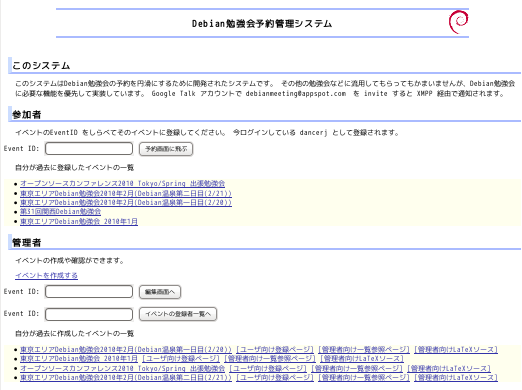
\includegraphics[width=0.5\hsize]{image201002/debianmeeting-screenshot.png}

\subsubsection{認証の仕組み}

このアプリケーションでは Google App Engine を利用しています。ユーザ認証は
Google App Engine で標準で提供されるGoogleの認証を流用しています。パスワー
ドの管理やユーザのメールアドレスの管理などをフレームワークに一任することで管理を
簡単にしています。


\subsubsection{データベースの構造}

バックエンドのデータベースには、AppEngineのDatastoreを利用しています。
Event と、 Attendance と UserRealName というのを定義しています。

Event は主催者がイベントについて登録した情報を保持しています。イベント毎
に存在しています。

Attendance はユーザがイベントに登録したという情報を保持しています。
イベントに対して登録したユーザの数だけ存在します。

UserRealname はユーザの表示名前の情報を保持しています。
各ユーザ毎に存在します。

\begin{commandline}

class Event(db.Model):
    eventid = db.StringProperty()
    owner = db.UserProperty() # the creator is the owner
    owners_email = db.StringListProperty() # allow owner emails to be added if possible
    title = db.StringProperty()
    location = db.StringProperty(multiline=True)
    content = db.StringProperty(multiline=True)
    content_url = db.StringProperty()
    prework = db.StringProperty(multiline=True)
    event_date = db.StringProperty()
    timestamp = db.DateTimeProperty(auto_now_add=True)
    capacity = db.IntegerProperty() # the number of possible people attending the meeting

class Attendance(db.Model):
    eventid = db.StringProperty()
    user = db.UserProperty()
    user_realname = db.StringProperty() # keep a cache of last realname entry.
    prework = db.StringProperty(multiline=True) # obsolete, but used in initial version
    prework_text = db.TextProperty() # Used everywhere, populate from prework if available.
    attend = db.BooleanProperty()
    enkai_attend = db.BooleanProperty()
    timestamp = db.DateTimeProperty(auto_now_add=True)

class UserRealname(db.Model):
    """Backup of user realname configuration so that user doesn't have to reenter that information."""
    user = db.UserProperty()
    realname = db.StringProperty()
    timestamp = db.DateTimeProperty(auto_now_add=True)

\end{commandline}

\subsubsection{ソースコードの構造}

ソースコードは現在下記の構成です。
\begin{itemize}
 \item \url{debianmeeting.py}: どのページがどのコードを呼び出すのかとい
       う部分を管理しているコードです。あと、どこに入れるのか迷ったコー
       ドもここにあるかも。
 \item \url{admin_event.py}: 主催者のイベントの管理関連のコードです。
 \item \url{user_registration.py}: ユーザの登録関連のコードです。
 \item \url{webapp_generic.py}: とりあえず共通のロジックを定義しています。
       POST と GET を同じように扱うためのコードなどが入っています。
 \item \url{schema.py}: データストアのスキーマが定義されています。
 \item \url{send_notification.py}: メール送信とXMPP送信ロジックが記述さ
       れています。
 \item \url{testSystem.py}: ユニットテストです。
\end{itemize}

ソース内部からテンプレートファイルが参照されています。

\begin{itemize}
 \item \url{EditEvent.html}
 \item \url{PreworkLatex.txt}
 \item \url{RegisterEvent.txt}
 \item \url{Thanks.html}
 \item \url{TopPage.html}
 \item \url{UserCommitEventRegistration.txt}
 \item \url{UserEventRegistrationPage.html}
 \item \url{UserEventRegistrationPage_Simple.html}
 \item \url{ViewEventSummary.html}
\end{itemize}

\subsubsection{ウェブページの遷移}

ウェブページの遷移とソースコードの対応をみてみます。

\includegraphics[width=1\hsize]{image201001/debian-reservation-flow.eps}


\subsection{今後の展望}


とりあえずは動いています。今後、何が変わるべきか。今後どういう点が実装さ
れるべきか。パッチウェルカム。



%\printindex

\cleartooddpage

\vspace*{15cm}
\hrule
\vspace{2mm}

\includegraphics[width=2cm]{image200502/openlogo-nd.eps}
\noindent \Large \bf Debian 勉強会資料\\ \\
\noindent \normalfont \debmtgyear{}年\debmtgmonth{}月\debmtgdate{}日 \hspace{5mm}  初版第1刷発行\\
\noindent \normalfont 東京エリア Debian 勉強会 (編集・印刷・発行)\\
\hrule

\end{document}
